%%
% Copyright (c) 2018, Pascal Wagler;  
% Copyright (c) 2014--2018, John MacFarlane
% 
% All rights reserved.
% 
% Redistribution and use in source and binary forms, with or without 
% modification, are permitted provided that the following conditions 
% are met:
% 
% - Redistributions of source code must retain the above copyright 
% notice, this list of conditions and the following disclaimer.
% 
% - Redistributions in binary form must reproduce the above copyright 
% notice, this list of conditions and the following disclaimer in the 
% documentation and/or other materials provided with the distribution.
% 
% - Neither the name of John MacFarlane nor the names of other 
% contributors may be used to endorse or promote products derived 
% from this software without specific prior written permission.
% 
% THIS SOFTWARE IS PROVIDED BY THE COPYRIGHT HOLDERS AND CONTRIBUTORS 
% "AS IS" AND ANY EXPRESS OR IMPLIED WARRANTIES, INCLUDING, BUT NOT 
% LIMITED TO, THE IMPLIED WARRANTIES OF MERCHANTABILITY AND FITNESS 
% FOR A PARTICULAR PURPOSE ARE DISCLAIMED. IN NO EVENT SHALL THE 
% COPYRIGHT OWNER OR CONTRIBUTORS BE LIABLE FOR ANY DIRECT, INDIRECT, 
% INCIDENTAL, SPECIAL, EXEMPLARY, OR CONSEQUENTIAL DAMAGES (INCLUDING,
% BUT NOT LIMITED TO, PROCUREMENT OF SUBSTITUTE GOODS OR SERVICES; 
% LOSS OF USE, DATA, OR PROFITS; OR BUSINESS INTERRUPTION) HOWEVER 
% CAUSED AND ON ANY THEORY OF LIABILITY, WHETHER IN CONTRACT, STRICT 
% LIABILITY, OR TORT (INCLUDING NEGLIGENCE OR OTHERWISE) ARISING IN 
% ANY WAY OUT OF THE USE OF THIS SOFTWARE, EVEN IF ADVISED OF THE 
% POSSIBILITY OF SUCH DAMAGE.
%%

%%
% For usage information and examples visit the GitHub page of this template:
% https://github.com/Wandmalfarbe/pandoc-latex-template
%%

\PassOptionsToPackage{unicode=true}{hyperref} % options for packages loaded elsewhere
\PassOptionsToPackage{hyphens}{url}
%
\documentclass[a4paper,,tablecaptionabove]{scrbook}
\usepackage{lmodern}
\usepackage{amssymb,amsmath}
\usepackage{ifxetex,ifluatex}
\usepackage{fixltx2e} % provides \textsubscript
\ifnum 0\ifxetex 1\fi\ifluatex 1\fi=0 % if pdftex
  \usepackage[T1]{fontenc}
  \usepackage[utf8]{inputenc}
  \usepackage{textcomp} % provides euro and other symbols
\else % if luatex or xelatex
  \usepackage{unicode-math}
  \defaultfontfeatures{Ligatures=TeX,Scale=MatchLowercase}
\fi
% use upquote if available, for straight quotes in verbatim environments
\IfFileExists{upquote.sty}{\usepackage{upquote}}{}
% use microtype if available
\IfFileExists{microtype.sty}{%
\usepackage[]{microtype}
\UseMicrotypeSet[protrusion]{basicmath} % disable protrusion for tt fonts
}{}
\IfFileExists{parskip.sty}{%
\usepackage{parskip}
}{% else
\setlength{\parindent}{0pt}
\setlength{\parskip}{6pt plus 2pt minus 1pt}
}
\usepackage{fancyvrb}
\usepackage{hyperref}
\hypersetup{
            pdftitle={A Client-side JavaScript Architecture},
            pdfauthor={Kevin Singer},
            pdfkeywords={some, nice, tags},
            pdfborder={0 0 0},
            breaklinks=true}
\urlstyle{same}  % don't use monospace font for urls
\VerbatimFootnotes % allows verbatim text in footnotes
\usepackage[margin=2.5cm,includehead=true,includefoot=true,centering]{geometry}
\usepackage{listings}
\newcommand{\passthrough}[1]{#1}
\usepackage{graphicx,grffile}
\makeatletter
\def\maxwidth{\ifdim\Gin@nat@width>\linewidth\linewidth\else\Gin@nat@width\fi}
\def\maxheight{\ifdim\Gin@nat@height>\textheight\textheight\else\Gin@nat@height\fi}
\makeatother
% Scale images if necessary, so that they will not overflow the page
% margins by default, and it is still possible to overwrite the defaults
% using explicit options in \includegraphics[width, height, ...]{}
\setkeys{Gin}{width=\maxwidth,height=\maxheight,keepaspectratio}
\setlength{\emergencystretch}{3em}  % prevent overfull lines
\providecommand{\tightlist}{%
  \setlength{\itemsep}{0pt}\setlength{\parskip}{0pt}}
\setcounter{secnumdepth}{5}
% Redefines (sub)paragraphs to behave more like sections
\ifx\paragraph\undefined\else
\let\oldparagraph\paragraph
\renewcommand{\paragraph}[1]{\oldparagraph{#1}\mbox{}}
\fi
\ifx\subparagraph\undefined\else
\let\oldsubparagraph\subparagraph
\renewcommand{\subparagraph}[1]{\oldsubparagraph{#1}\mbox{}}
\fi

% Make use of float-package and set default placement for figures to H
\usepackage{float}
\floatplacement{figure}{H}

\makeatletter
\@ifpackageloaded{subfig}{}{\usepackage{subfig}}
\@ifpackageloaded{caption}{}{\usepackage{caption}}
\captionsetup[subfloat]{margin=0.5em}
\AtBeginDocument{%
\renewcommand*\figurename{Figure}
\renewcommand*\tablename{Table}
}
\AtBeginDocument{%
\renewcommand*\listfigurename{List of Figures}
\renewcommand*\listtablename{List of Tables}
}
\newcommand*\listoflistings\lstlistoflistings
\AtBeginDocument{%
\renewcommand*{\lstlistlistingname}{List of Listings}
}
\makeatother

\title{A Client-side JavaScript Architecture}
\providecommand{\subtitle}[1]{}
\subtitle{For the Web-of-Needs Owner-Application Prototype}
\author{Kevin Singer}
\date{25.01.2018}





%%
%% added
%%

%
% No language specified? take American English.
%

\ifnum 0\ifxetex 1\fi\ifluatex 1\fi=0 % if pdftex
  \usepackage[shorthands=off,main=english]{babel}
\else
    % See issue https://github.com/reutenauer/polyglossia/issues/127
  \renewcommand*\familydefault{\sfdefault}
    % load polyglossia as late as possible as it *could* call bidi if RTL lang (e.g. Hebrew or Arabic)
  \usepackage{polyglossia}
  \setmainlanguage[]{english}
\fi


%
% colors
%
\usepackage[dvipsnames,svgnames*,x11names*,table]{xcolor}

%
% listing colors
%
\definecolor{listing-background}{HTML}{F7F7F7}
\definecolor{listing-rule}{HTML}{B3B2B3}
\definecolor{listing-numbers}{HTML}{B3B2B3}
\definecolor{listing-text-color}{HTML}{000000}
\definecolor{listing-keyword}{HTML}{435489}
\definecolor{listing-identifier}{HTML}{435489}
\definecolor{listing-string}{HTML}{00999A}
\definecolor{listing-comment}{HTML}{8E8E8E}
\definecolor{listing-javadoc-comment}{HTML}{006CA9}

%\definecolor{listing-background}{rgb}{0.97,0.97,0.97}
%\definecolor{listing-rule}{HTML}{B3B2B3}
%\definecolor{listing-numbers}{HTML}{B3B2B3}
%\definecolor{listing-text-color}{HTML}{000000}
%\definecolor{listing-keyword}{HTML}{D8006B}
%\definecolor{listing-identifier}{HTML}{000000}
%\definecolor{listing-string}{HTML}{006CA9}
%\definecolor{listing-comment}{rgb}{0.25,0.5,0.35}
%\definecolor{listing-javadoc-comment}{HTML}{006CA9}

%
% for the background color of the title page
%
\usepackage{pagecolor}
\usepackage{afterpage}

%
% TOC depth and 
% section numbering depth
%
\setcounter{tocdepth}{3}
\setcounter{secnumdepth}{3}

%
% line spacing
%
\usepackage{setspace}
\setstretch{1.2}

%
% break urls
%
\PassOptionsToPackage{hyphens}{url}

%
% When using babel or polyglossia with biblatex, loading csquotes is recommended 
% to ensure that quoted texts are typeset according to the rules of your main language.
%
\usepackage{csquotes}

%
% captions
%
\definecolor{caption-color}{HTML}{777777}
\usepackage[font={stretch=1.2}, textfont={color=caption-color}, position=top, skip=4mm, labelfont=bf, singlelinecheck=false, justification=raggedright]{caption}
\setcapindent{0em}
\captionsetup[longtable]{position=above}

%
% blockquote
%
\definecolor{blockquote-border}{RGB}{221,221,221}
\definecolor{blockquote-text}{RGB}{119,119,119}
\usepackage{mdframed}
\newmdenv[rightline=false,bottomline=false,topline=false,linewidth=3pt,linecolor=blockquote-border,skipabove=\parskip]{customblockquote}
\renewenvironment{quote}{\begin{customblockquote}\list{}{\rightmargin=0em\leftmargin=0em}%
\item\relax\color{blockquote-text}\ignorespaces}{\unskip\unskip\endlist\end{customblockquote}}

%
% Source Sans Pro as the de­fault font fam­ily
% Source Code Pro for monospace text
%
% 'default' option sets the default 
% font family to Source Sans Pro, not \sfdefault.
%
\usepackage[default]{sourcesanspro}
\usepackage{sourcecodepro}

%
% heading color
%
\definecolor{heading-color}{RGB}{40,40,40}
\addtokomafont{section}{\color{heading-color}}
% When using the classes report, scrreprt, book, 
% scrbook or memoir, uncomment the following line.
%\addtokomafont{chapter}{\color{heading-color}}

%
% variables for title and author
%
\usepackage{titling}
\title{A Client-side JavaScript Architecture}
\author{Kevin Singer}

%
% tables
%

%
% remove paragraph indention
%
\setlength{\parindent}{0pt}
\setlength{\parskip}{6pt plus 2pt minus 1pt}
\setlength{\emergencystretch}{3em}  % prevent overfull lines

%
%
% Listings
%
%

\lstdefinestyle{eisvogel_listing_style}{
  language         = java,
  numbers          = left,
  backgroundcolor  = \color{listing-background},
  basicstyle       = \color{listing-text-color}\small\ttfamily{}\linespread{1.15}, % print whole listing small
  xleftmargin      = 2.7em,
  breaklines       = true,
  frame            = single,
  framesep         = 0.6mm,
  rulecolor        = \color{listing-rule},
  frameround       = ffff,
  framexleftmargin = 2.5em,
  tabsize          = 4,
  numberstyle      = \color{listing-numbers},
  aboveskip        = 1.0em,
  keywordstyle     = \color{listing-keyword}\bfseries,
  classoffset      = 0,
  sensitive        = true,
  identifierstyle  = \color{listing-identifier},
  commentstyle     = \color{listing-comment},
  morecomment      = [s][\color{listing-javadoc-comment}]{/**}{*/},
  stringstyle      = \color{listing-string},
  showstringspaces = false,
  escapeinside     = {/*@}{@*/}, % Allow LaTeX inside these special comments
  literate         =
  {á}{{\'a}}1 {é}{{\'e}}1 {í}{{\'i}}1 {ó}{{\'o}}1 {ú}{{\'u}}1
  {Á}{{\'A}}1 {É}{{\'E}}1 {Í}{{\'I}}1 {Ó}{{\'O}}1 {Ú}{{\'U}}1
  {à}{{\`a}}1 {è}{{\'e}}1 {ì}{{\`i}}1 {ò}{{\`o}}1 {ù}{{\`u}}1
  {À}{{\`A}}1 {È}{{\'E}}1 {Ì}{{\`I}}1 {Ò}{{\`O}}1 {Ù}{{\`U}}1
  {ä}{{\"a}}1 {ë}{{\"e}}1 {ï}{{\"i}}1 {ö}{{\"o}}1 {ü}{{\"u}}1
  {Ä}{{\"A}}1 {Ë}{{\"E}}1 {Ï}{{\"I}}1 {Ö}{{\"O}}1 {Ü}{{\"U}}1
  {â}{{\^a}}1 {ê}{{\^e}}1 {î}{{\^i}}1 {ô}{{\^o}}1 {û}{{\^u}}1
  {Â}{{\^A}}1 {Ê}{{\^E}}1 {Î}{{\^I}}1 {Ô}{{\^O}}1 {Û}{{\^U}}1
  {œ}{{\oe}}1 {Œ}{{\OE}}1 {æ}{{\ae}}1 {Æ}{{\AE}}1 {ß}{{\ss}}1
  {ç}{{\c c}}1 {Ç}{{\c C}}1 {ø}{{\o}}1 {å}{{\r a}}1 {Å}{{\r A}}1
  {€}{{\EUR}}1 {£}{{\pounds}}1 {«}{{\guillemotleft}}1
  {»}{{\guillemotright}}1 {ñ}{{\~n}}1 {Ñ}{{\~N}}1 {¿}{{?`}}1
  {…}{{\ldots}}1 {≥}{{>=}}1 {≤}{{<=}}1 {„}{{\glqq}}1 {“}{{\grqq}}1
  {”}{{''}}1
}
\lstset{style=eisvogel_listing_style}

\lstdefinelanguage{XML}{
  morestring      = [b]",
  moredelim       = [s][\bfseries\color{listing-keyword}]{<}{\ },
  moredelim       = [s][\bfseries\color{listing-keyword}]{</}{>},
  moredelim       = [l][\bfseries\color{listing-keyword}]{/>},
  moredelim       = [l][\bfseries\color{listing-keyword}]{>},
  morecomment     = [s]{<?}{?>},
  morecomment     = [s]{<!--}{-->},
  commentstyle    = \color{listing-comment},
  stringstyle     = \color{listing-string},
  identifierstyle = \color{listing-identifier}
}

%
% header and footer
%
\usepackage{fancyhdr}
\pagestyle{fancy}
\fancyhead{}
\fancyfoot{}
\lhead{A Client-side JavaScript Architecture}
\chead{}
\rhead{25.01.2018}
\lfoot{Kevin Singer}
\cfoot{}
\rfoot{\thepage}
\renewcommand{\headrulewidth}{0.4pt}
\renewcommand{\footrulewidth}{0.4pt}

%%
%% end added
%%

\begin{document}

%%
%% begin titlepage
%%

\begin{titlepage}
\newgeometry{left=6cm}
\definecolor{titlepage-color}{HTML}{06386E}
\newpagecolor{titlepage-color}\afterpage{\restorepagecolor}
\newcommand{\colorRule}[3][black]{\textcolor[HTML]{#1}{\rule{#2}{#3}}}
\begin{flushleft}
\noindent
\\[-1em]
\color[HTML]{FFFFFF}
\makebox[0pt][l]{\colorRule[FFFFFF]{1.3\textwidth}{1pt}}
\par
\noindent

{ \setstretch{1.4}
\vfill
\noindent {\huge \textbf{\textsf{A Client-side JavaScript Architecture}}}
\vskip 1em
{\Large \textsf{For the Web-of-Needs Owner-Application Prototype}}
\vskip 2em
\noindent
{\Large \textsf{Kevin Singer}
\vfill
}

\textsf{25.01.2018}}
\end{flushleft}
\end{titlepage}
\restoregeometry

%%
%% end titlepage
%%


{
\setcounter{tocdepth}{2}
\tableofcontents
}
\listoftables
\listoffigures
\lstlistoflistings

\hypertarget{authorship-declaration}{%
\chapter{Authorship Declaration}\label{authorship-declaration}}

Hereby I declare, that I authored this work on my own and that all
sources and aids have been listed in their entirety and that all parts
of the work -- including tables, maps and figures -- stemming from other
works in exact wording or spirit, have been marked as quote and contain
a reference to the source.

\hypertarget{sec:abstract}{%
\chapter{Abstract}\label{sec:abstract}}

This thesis is part of the over-arching Web of Needs (see ref.
``Webofneeds'' \protect\hyperlink{ref-Webofneeds}{n.d.}; for related
publications see ref. ``Web of Needs Publications List''
\protect\hyperlink{ref-WebNeedsPublications2013}{2013}) project -- short
WoN -- and, somewhat more particular, of developing an end-user-friendly
client-application (see ref. ``Mat(ch)²at''
\protect\hyperlink{ref-Match}{n.d.}) prototype/demonstrator for it, that
allows testing the protocol and helps with communicating the WoN's
potential to people. The main focus of the work done for this thesis was
to research ways of structuring the JavaScript-based client-application;
thus it consisted of researching and experimenting with state-of-the-art
web-application architectures and tooling, adapting and innovating on
them for the particular problem space layed out in chapter
\ref{sec:probdescr}, as well as identifying a migration path for
updating the existing code-base.

As layed out in chapter \ref{sec:suggested-solution}, we used a variant
of the (ng-)redux architecture (see
secs.~\ref{sec:redux}, \ref{sec:ng-redux} for the original
architecture), but added a \enquote{messaging-agent} more akin to the
runtime in the Elm-architecture (see sec.~\ref{sec:elm-architecture}).
The action-creators, who handle non-socket network communication, use an
RDF-store for caching the RDF-data used throughout the Web of Needs. To
allow using newer language features and bundle the application Webpack
(sec.~\ref{sec:webpack}) with Babel (sec.~\ref{sec:cross-compilation})
is used. Styling is done in SCSS (sec.~\ref{sec:scss}) using BEM
(sec.~\ref{sec:TODO}) as naming convention.

\hypertarget{sec:intro}{%
\chapter{Introduction}\label{sec:intro}}

\hypertarget{sec:probdescr}{%
\chapter{Problem Description}\label{sec:probdescr}}

As mentioned already in the abstract, the challenge to be tackled by
this work was to find (and adapt) a state-of-the-art architecture and
tooling for the Web of Needs Owner client application and a migration
path of the JavaScript code-base to these, while addressing the
requirements layed out in this chapter. To define said requirements, we
first need to take a high-level look at what the Web of Needs is and how
people can interact with it.

\hypertarget{sec:web-of-needs}{%
\section{Web of Needs}\label{sec:web-of-needs}}

It is a set of protocols (and reference implementations) that allow
posting documents, for instance describing supply and demand. Starkly
simplified examples would be \enquote{I have a couch to give away} or
\enquote{I'd like to travel to Paris in a week and need transportation}.
These documents, called \enquote{needs} can be posted on arbitrary data
servers (called \enquote{WoN-Nodes}). There they're discovered by
matching-services, that continuously crawl the nodes they can find.
Additionally, to get results more quickly, nodes can notify matchers of
new needs. These then get compared with the ones the matcher already
knows about. If it finds a good pair -- e.g. \enquote{I have a couch to
give away} and \enquote{Looking for furniture for my living room} -- the
matcher notifies the owners of these needs. They can then decide whether
they want to contact each other. If they send and accept each other's
contact request, they can start chatting with each other. The protocol
in theory can also be used as a base-level for other interactions, like
entering into contracts or transferring money.

\hypertarget{sec:data-on-won-nodes}{%
\section{Data on WoN-Nodes}\label{sec:data-on-won-nodes}}

Needs, connections between them and any events on those connections are
published on the WoN-Nodes in the form of RDF, which stands for Resource
Description Framework (see ref. ``Resource Description Framework''
\protect\hyperlink{ref-ResourceDescriptionFramework}{n.d.}). In RDF,
using a variety of different syntax-alternatives, data is structured as
a graph that can be distributed over multiple (physical) resources.
Every graph-edge is defined by a subject (the start-node), a predicate
(the \enquote{edge-type}) and object (the target-node).

Note that the subject always needs to be an Unique Resource Identifiers
(URIs). For the case, when those URIs are also Uniform Resource Locators
(URLs) there is the convention to host that data under that URL. This
allows easily linking data graphs on multiple servers, thus making them
Linked Data (see ref. ``Linked Data''
\protect\hyperlink{ref-Linkeddata}{n.d.}). This is a necessary
requirement for the Web of Needs, as data is naturally spread out across
several servers, i.e.~WoN-Nodes.

Some example triples taken from a need/post on the WoN-Node running at
\url{http://node.matchat.org/resource/} (accessed 2018-06-18) could look
something like the following ones:

\begin{lstlisting}[caption={Excerpt of a need description (N-Triples)}, label=fig:needtriples]
<https://node.matchat.org/won/resource/need/ow14asq0gqsb>
<http://purl.org/webofneeds/model#is>
_:b0 .

<https://node.matchat.org/won/resource/need/ow14asq0gqsb>
<http://www.w3.org/1999/02/22-rdf-syntax-ns#type>
<http://purl.org/webofneeds/model#Need> .

_:b0
<http://purl.org/dc/elements/1.1/title>
"Simple easel to give away" .

_:b0
<http://purl.org/dc/elements/1.1/description>
"I've got an old easel lying around at my place that is \
mostly just catching dust. If there is any aspiring landscape \
painters that would like to have it: poke me :)" .
\end{lstlisting}

As can be seen, this way of specifying triples, called N-Triples, isn't
well-suited for direct reading or authoring; the subjects
(\passthrough{\lstinline!.../need/ow14asq0gqsb!} and
\passthrough{\lstinline!\_:b0!}) are repeated and large parts of the
URIs are duplicate. The short URIs starting with an underscore (e.g.
\passthrough{\lstinline!\_:b0!} are called blank-nodes and don't have
meaning outside of a document and can reoccur in other documents as
opposed to Unique Resource Identifiers. there is also a convention that
when using URLs used as subject-URIs (e.g.
\url{https://node.matchat.org/won/resource/need/ow14asq0gqsb}) it should
be possible to access these to get a document with the triples for that
subject.

There are several other markup-languages respectively
serialization-formats for easier writing and clearer serializations for
these triples, e.g.~Turtle/Trig, JSON-LD and the somewhat verbose
RDF/XML. The same example, but in JavaScript Object Notation for Linked
Data (JSON-LD) would read as follows:

\begin{lstlisting}[caption={Excerpt of a need description (JSON-LD)}, label=fig:needjson]
{
  "@id": "need:ow14asq0gqsb",
  "@type": "won:Need",
  "won:is": {
    "@id": "_:b3", // <-- optional
    "dc:title": "Simple easel to give away"
    "dc:description": "I've got an old easel lying \
    around at my place that is mostly just catching \
    dust. If there is any aspiring landscape painters \
    that would like to have it: poke me :)",
  },

  "@context": {
    "dc": "http://purl.org/dc/elements/1.1/",
    "need": "https://node.matchat.org/won/resource/need/",
    "won": "http://purl.org/webofneeds/model#"
  }
}
\end{lstlisting}

As can be seen above, JSON-LD allows to visually represent the nesting
(\passthrough{\lstinline!need:ow14asq0gqsb won:is \_:b3!}) and to define
prefixes (in the \passthrough{\lstinline!@context!}). Together this
allows to avoid redundancies. The other serialization-formats are
similar in this regard (and are used between other services in the Web
of Needs) -- see below for a turtle-serialization of the same triples:

\begin{lstlisting}[caption={Excerpt of a need description (TTL)}, label=fig:needttl]
@prefix dc:    <http://purl.org/dc/elements/1.1/> .
@prefix need:  <https://node.matchat.org/won/resource/need/> .
@prefix won:   <http://purl.org/webofneeds/model#> .

need:ow14asq0gqsb
  a             won:Need ;
  won:is        [
    dc:title         "Simple easel to give away" ;
    dc:description   "I've got an old easel lying
      around at my place that is mostly just catching
      dust. If there is any aspiring landscape painters
      that would like to have it: poke me :)"
  ]
\end{lstlisting}

However, as JSON-LD also constitutes valid
JSON/JS-object-literal-syntax, it is the natural choice for using it in
the JS-based client-application and was already being used in the
existing code-base.

\hypertarget{sec:won-owner-application}{%
\section{WoN-Owner-Application}\label{sec:won-owner-application}}

\hypertarget{sec:interaction-design}{%
\subsection{Interaction Design}\label{sec:interaction-design}}

Among the three services that play roles in the web of needs --
matchers, nodes and owner-applications -- the work at hand has its focus
on the latter of these. It provides people with a way to interact with
the other services in a similar way to how an email-client allows
interacting with email-servers. Through it, people can:

\begin{itemize}
\tightlist
\item
  Create and post new needs. Currently these consist of a simple
  data-structure with a subject line, a long textual description and
  optional tags or location information.
\item
  View needs/posts and all data in them in a human-friendly fashion
\item
  Share links to needs/posts with other people
\item
  Immediately get notified of and see matches, incoming requests and
  chat messages
\item
  Send and accept contact/connection requests
\item
  Write and send chat messages
\end{itemize}

For exploring these interactions, several prototypes had already been
designed and implemented. The first were paper-based or simple clickable
dummies, that weren't fully interactive. The last prototype before the
one described in this work had been implemented using Angular 1.X and
its MVC-architecture (sec.~\ref{sec:angular-mvc}). For this iteration
new graphic designs were made, that necessesitated to leave the
Bootstrap-theme we had previously been using behind and develop and
maintain our own (S)CSS (see section \ref{sec:scss}).

\hypertarget{sec:technical-requirements}{%
\subsection{Technical Requirements}\label{sec:technical-requirements}}

On the development-side of things, the requirements were:

\begin{itemize}
\tightlist
\item
  The application needs to be able to keep data in sync between
  browser-tabs running the JS-client and the Java-based servers. This
  happens through a REST-API and websockets. Most messages arrive at the
  WoN-Owner-Server from the WoN-Node and just get forwarded to the
  client via the websocket. The only data directly stored on and fetched
  from the Owner-Server are the URIs and private keys{[}\^{}cryptography
  happens on the WoN-Owner-Server{]} of needs/posts owned by an account,
  as well as information which messages have been seen. All other data
  lives on the WoN-Node-Servers, that have no concept of user-accounts.
\item
  As subject of a research-project, the protocols can change at any
  time. Doing so should only cause minimal refactoring in the
  owner-application.
\item
  In the future different means of protocols will be added to
  connections, i.e.~interactions between needs, such as payments or the
  recently added \enquote{agreements}, i.e.~a mechanism to make
  formalized contracts via messages exchanged over the connections by
  formally agreeing with the contents of other messages)
\item
  Ultimately the interface for authoring needs should support a wide
  range of ontologies\footnote{Ontologies can be described as
    data-structure-descriptions, i.e.~schemata, for RDF-data. E.g. the
    current demo-ontology defines that needs can have a title, a
    description, a location, tags, etc.} respectively any ontology
  people might want to use for describing things and concepts. Adapting
  the authoring GUIs or even just adding a few form input widgets should
  be seamless and only require a few local changes.
\item
  We\footnote{My colleagues at the researchstudio Smart Agent
    Technologies and I} didn't want to deal with the additional
  hurdles/constraints of designing the prototype for mobile-screens at
  first, but a later adaption/port was to be expected. Changing the
  client application for that needed to require minimal effort.
\item
  It should be possible to build an application that feels responsive
  when using it. This means low times till first meaningful render and
  complete page-load. This in term implies a reduction of round-trips
  and HTTP-requests and use of caching mechanisms for data and
  application code. But \enquote{feeling responsive} also means that
  operations that take a while despite all other efforts need to show
  feedback to the user (e.g.~spinning wheels, progress bars, etc) to
  communicate that the application hasn't frozen.
\item
  Runs on ever-green browsers. As it's a research-prototype there is
  less need to support old browsers, like the pre-edge
  internet-explorer.
\item
  Good developer experience, i.e.~new language features to allow more
  expressive, robust and concise code, warnings about possible bugs
  where possible, auto-completion, jump-to-definition, documentation on
  mouse-hover, etc.
\item
  Any new technologies needed to be feasible to learn within the
  project's scope.
\item
  The more of the old code-base that could be kept, the better in regard
  to the scope.
\end{itemize}

The previous iteration of the prototype had already been implemented in
Angular-js 1.X. However, the code-base was proving hard to maintain. We
continuously had to deal with bugs that were hard to track down, partly
because JavaScript's dynamic nature obscured where they originated in
the code and mostly because causality in the Angular-app became
increasingly convoluted and hard to understand. The application's
architecture needed an overhaul to deal with these issues, which gave
rise to the work at hand. Thus, additional requirements were:

\begin{itemize}
\tightlist
\item
  Causality in the application is clear and concise to make
  understanding the code and tracking down bugs easier.
\item
  Local changes can't break code elsewhere, i.e.~side-effects are
  minimized.
\item
  Responsibilities of functions and classes are clear and separated, so
  that multiple developers can easily collaborate.
\item
  The current system state is transparent and easily understandable to
  make understanding causality easier.
\item
  The solution should lessen the problems that JavaScript's weakly-typed
  nature causes, e.g.~bugs causing errors way later in the program-flow
  instead of at the line where the problem lies.
\item
  Reduces code-redundancies
\item
  Makes code conciser and clearer to the reader
\end{itemize}

\hypertarget{sec:state-of-the-art}{%
\chapter{State of the Art}\label{sec:state-of-the-art}}

\hypertarget{frameworks-and-architecture}{%
\section{Frameworks and
Architecture}\label{frameworks-and-architecture}}

The following patterns all help with developing graphical user
interfaces, by providing separation of concerns and decoupling. This
makes it easier for multiple developers to collaborate and allows better
reasoning about the app's behaviour. It also makes adapting the
application easier when the understaning of the design problem changes.

The presented architectural patterns for client-side
JavaScript-applications, at the time of writing encompass all widely
used and sufficiently distinct I could discern during my technology- and
literature research. This selection provides the reference for choosing
an architecture for the Web of Needs owner application, which
architecture is based off of redux (sec.~\ref{sec:redux}) in general and
ng-redux (sec.~\ref{sec:ng-redux}) in particular. The reasons for this
design-decision will be discussed in section
\ref{sec:suggested-solution} \enquote{Suggested Solution}.

\hypertarget{sec:mvc}{%
\subsection{Model-View-Controller}\label{sec:mvc}}

On of the, if not the most classical architectural pattern typically
used in frontend-programming is Model-View-Controller. It was first
introduced in the 70s at the Palo Alto Research Center (Reenskaug
\protect\hyperlink{ref-ReenskaugThingModelViewEditor1979}{1979}) and
first formally published by Krasner and Pope
(\protect\hyperlink{ref-KrasnerCookbookUsingModelview1988}{1988}\protect\hyperlink{ref-KrasnerCookbookUsingModelview1988}{b}).
As it's still widely used and angular's MVC (sec.~\ref{sec:angular-mvc})
is a variant thereof it shall be shortly described here for the sake of
completeness. The pattern mainly consists of three types of building
blocks (as can also be seen in figure fig.~\ref{fig:mvc}):

\begin{itemize}
\tightlist
\item
  \textbf{controllers} contain the lion's share of the business logic.
  User input gets handled by them and they get to query the model.
  Depending on these two information sources they decide what messages
  to send to the the model, i.e.~the controller telling the model to
  change. Usually there is one controller per view and vice-versa.
\item
  \textbf{models} hold the application's state and make sure it's
  consistent. If something in the data changes, it notifies views and
  controllers depending on it. These notifications can be parametrized,
  telling the dependants what changed.
\item
  \textbf{views} are what the outside world/user's get to see. When the
  model changes, the view get's notified and -- depending on the data
  passed along and what it reads from the model -- updates accordingly.
  Especially in HTML-applications, views (and thereby controllers) tend
  to be nested (e.g.~the entire screen -- a column -- a widget in it --
  a button in the widget)
\end{itemize}

Note, that there is a wide range of different interpretations of this
architectural pattern, that organise models, views and controllers
differently. Section \ref{sec:angular-mvc} describes one of these
(angular 1.X' MVC) in more detail.

\begin{figure}
\hypertarget{fig:mvc}{%
\centering
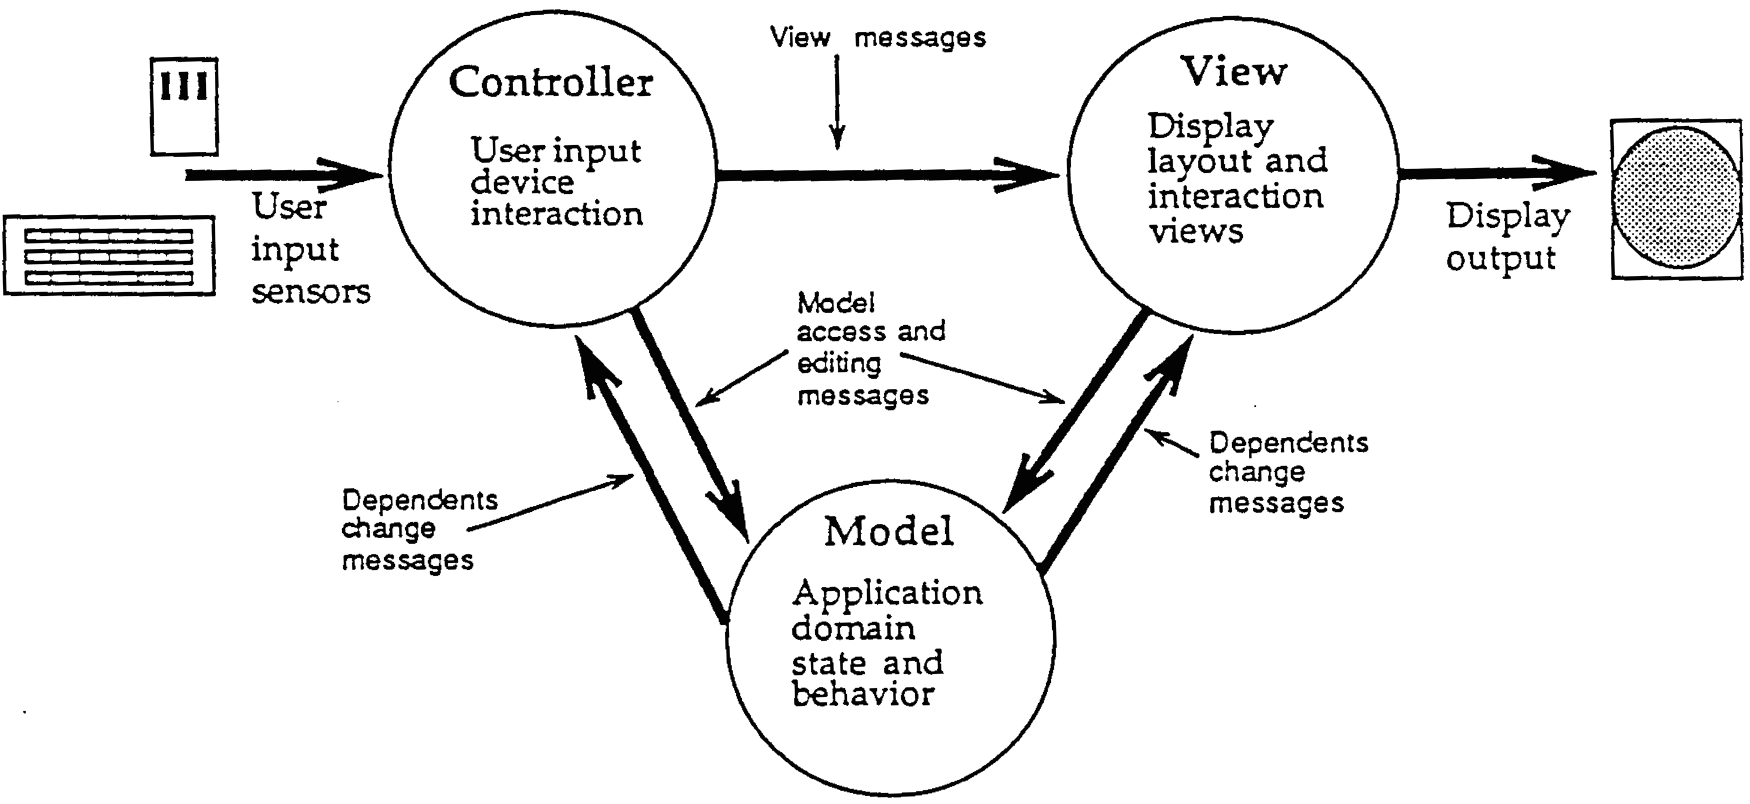
\includegraphics{./tex2pdf.11982/4392ac73b7368e734eb911fc5ec7524829e995aa.png}
\caption{MVC-architecture (Krasner and Pope
\protect\hyperlink{ref-Krasnerdescriptionmodelviewcontrolleruser1988}{1988}\protect\hyperlink{ref-Krasnerdescriptionmodelviewcontrolleruser1988}{a})}\label{fig:mvc}
}
\end{figure}

\hypertarget{sec:mvvm}{%
\subsection{Model-View-ViewModel}\label{sec:mvvm}}

This architectural pattern, also known as \enquote{Model-View-Binder} is
similar to MVC but puts more emphasis on the separation between back-end
and front-end. Its parts are the following (see also
fig.~\ref{fig:mvvm}):

\begin{itemize}
\tightlist
\item
  \textbf{The model} is the back-end business-logic and state. It can be
  on a different machine entirely, e.g.~a web server.
\item
  \textbf{The view-model} contains the front-end logic and state. It is
  a thin binding layer, that processes inputs and that manages and
  provides the data required by the view.
\item
  \textbf{The view} is a stateless rendering of the data retrieved from
  the view-model; in the case of some frameworks, this happens via
  declarative statements in the view's templates, that automatically get
  updated when the data in the view-model changes. User-input events
  raised in the view get forwarded to the view-model.
\end{itemize}

\begin{figure}
\hypertarget{fig:mvvm}{%
\centering
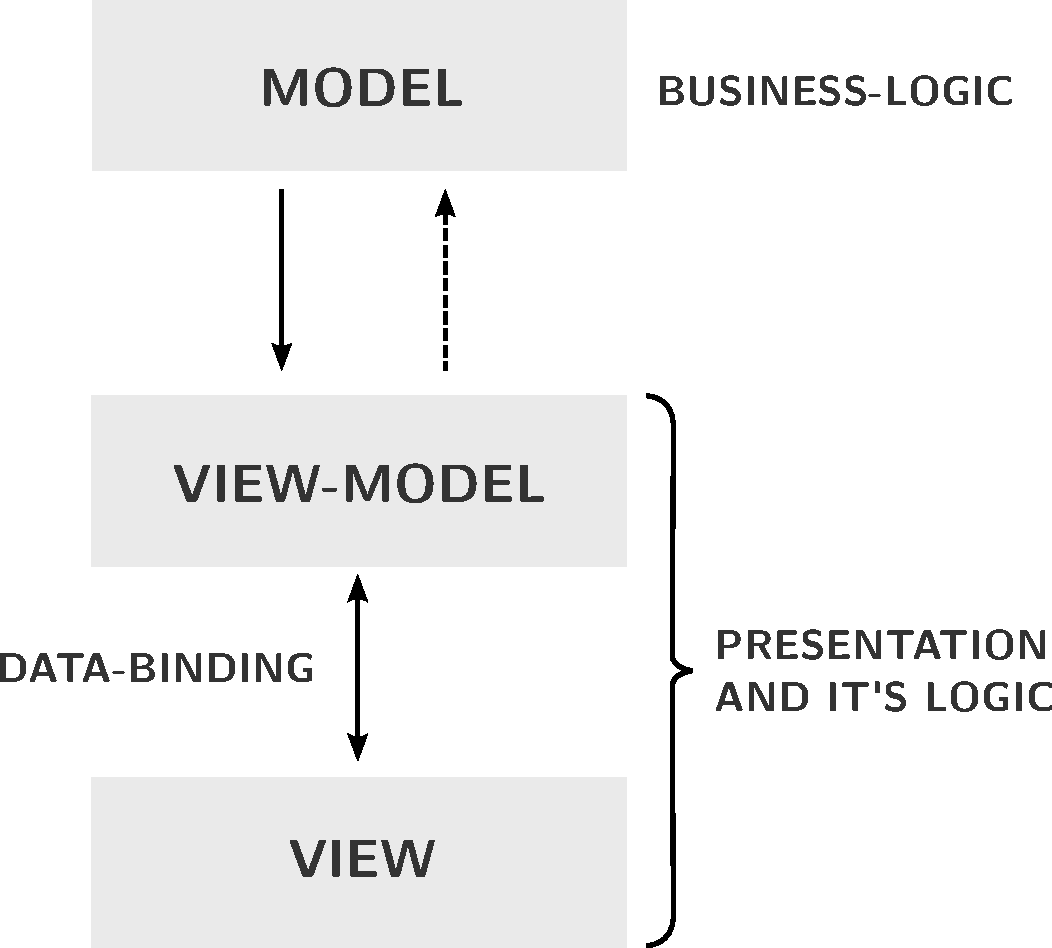
\includegraphics[width=\textwidth,height=8cm]{./tex2pdf.11982/a9215b936073b90bd24770863c82edb8b1c0c75f.pdf}
\caption{MVVM-architecture (source:
\url{https://en.wikipedia.org/wiki/File:MVVMPattern.png}, accessed
2018-06-18)}\label{fig:mvvm}
}
\end{figure}

\hypertarget{sec:angular-mvc}{%
\subsection{Angular 1.x MVC}\label{sec:angular-mvc}}

Angular 1.x is a JavaScript-framework that roughly follows the MVC/MVVM
architectures, but has a few conceptual variations and extensions.

For views it uses a template-syntax. See the following snippet for an
exmple from the webofneeds-codebase, that renders to an
\passthrough{\lstinline!<h2>!}-header and a paragraph with a
description, if the description is present (the
\passthrough{\lstinline!ng-show!} is a conditional):

\begin{lstlisting}[language=HTML, caption={Example angular template code from WoN-codebase}, label=fig:ng-template]
...
<h2 class="post-info__heading"
  ng-show="self.post.getIn([
    'won:hasContent','won:hasTextDescription'
  ])">
    Description
</h2>
<p class="post-info__details"
  ng-show="self.post.getIn([
    'won:hasContent','won:hasTextDescription'
  ])">
    {{ self.post.getIn(['won:hasContent','won:hasTextDescription']) }}
</p>
...
\end{lstlisting}

These are either specified in an HTML-file and then later linked with a
controller or are a string in the declaration of something called a
\enquote{directive} (which are custom HTML tags or properties). Every
template has a scope object bound to it and can contain expressions --
e.g.~those in curly braces -- that have access to that scope object. For
the code-example in above this means, that -- in the HTML that the user
gets to see -- the curly braces will have been replaced by the result of
\passthrough{\lstinline!self.post.getIn(['won:hasContent','won:hasTextDescription'])!}
(the \passthrough{\lstinline!getIn!} is there because
\passthrough{\lstinline!post!} is an immutable-js (see ref.
``Immutable.js'' \protect\hyperlink{ref-Immutablejs}{n.d.}) object).
Practically every time the result of that expression changes, angular
will update the displayed value. Basically every expression causes a
\enquote{watch} to be created (this can also be done manually via
\passthrough{\lstinline!$scope.watch!}). During what's called a
\enquote{digest-cycle} it checks all of these watch-expressions for
changes and then executes their callbacks, which in the case of the
curly-braces causes the DOM-update. These digest-cycles are triggered by
a lot of provided directives or if you call the function
\passthrough{\lstinline!$apply!}. Some thought needs to be given to
managing these to avoid imperformance and also because you can't call
\passthrough{\lstinline!$apply!} while already in a digest-cycle.

Beyond the curly braces, angular also provides a handful of other
template-utilities in the form of directives. For instance the
property-directive \passthrough{\lstinline!ng-repeat!} allows iterating
over a collection as follows:

\passthrough{\lstinline!\{fig:ng-repeat .html caption="Example ng-repeat usage"\} <div ng-repeat="el in collection">\{\{el.someVar\}\}</div>!}

Or, similarly, \passthrough{\lstinline!ng-show="someBoolVar"!}
conditionally displays content.

Note that these template-bindings are bi-directional, i.e.~the code in
the template can change the the values in the model (the template's
\enquote{scope}). Additionally, templates/directives can be nested
within each other. By default, their scopes then use JavaScript's
prototypical inheritance (see ref. ``Inheritance and the Prototype
Chain'' \protect\hyperlink{ref-Inheritanceprototypechain}{n.d.})
mechanism, i.e.~if a value can't be found on the template's/directive's
scope, angular will then go on to try to get it from the on the one
wrapping it (and so on) This allows writing small apps or components
where all data-flows are represented and all code contained in the
template. For medium-sized or large apps however, the combination of
bi-directional binding and scope inheritance, can lead to hard-to-follow
causality, thus hard-to-track-down bugs and thus poor maintainability.
More on that later in (section {\textbf{???}}).

Also, using scope inheritance reduces reusability, as the respective
components won't work in other contexts anymore.

For all but the very smallest views/components the UI-update logic will
be contained in angular's controllers, however. They are connected with
their corresponding templates via the routing-configuration (more on
that later in section \ref{sec:ref-to-routing-subsection}) or by being
part of the same directive (see
sec.~\ref{sec:ref-to-directive-subsection}). Controllers have access to
their template's scope and vice versa
(sec.~\ref{sec:controllerAs-discussion})

Theoretically, it's possible to reuse controllers with different
templates, but this can lead to hard-to-track-down and I'd advise
against doing that. When nesting templates and thus their associated
controllers, the latter form something like a prototypical inheritance
chain: If a variable isn't found on the controller, respectively its
scope, the default is to check on its parent and its parent's parent,
etc, up to the root-scope. Note, that scopes can be defined as isolated
(sec.~\ref{sec:ref-to-routingux2fdirectiveux2fisolated-scope-section})
-- for views in their routing configuration and for directives in their
declaration. This allows to avoid this behavior, which I'd recommend for
predicatability- and thus maintainability-reasons.

These scopes (models), templates (views) and controllers constitute a
classical MVC-architecture (see section \ref{sec:mvc}). However, angular
also has the concept of services: Essentially, they are objects that
controllers can access and that can provide utility functions, manage
global application state or make HTTP requests to a web server.
Controllers can't gain access to each other -- except for nesting /
prototypical inheritance -- but they can always request access to any
service (via dependency injection; more on that later in section
\ref{sec:TODO}). Examples of services are, for instance,
\passthrough{\lstinline!$scope!} that, amongst others, allows
registering custom watch-expressions with angular outside of templates,
like so:

\begin{lstlisting}[caption={Example of listening for changes of a variable in angular}, label=fig:ng-simple-ctrl]
var myApp = angular.module('myApp', []);
myApp.controller('PostController', function ($scope) {
  $scope.post = { text: 'heio! :)' };
  $scope.$watch('post.text', function(currentText, prevText) {
    console.log('Text has been edited: ', currentText);
  });
});
\end{lstlisting}

Another example for a service would be
\passthrough{\lstinline!linkeddata-service.js!} that had already been
written for the first won-owner-application protototype and that is
still in use. It can be used to load and cache RDF-data\footnote{see
  section \ref{sec:data-on-won-nodes} for more on RDF}.

Considering services, it's the angular framework can also be viewed
through the lense of MVVM (see section \ref{sec:mvvm}), with templates
as views, scopes and controllers as view-models and services as models
or as proxies for models on a web server (as we did with
\passthrough{\lstinline!linkeddata-service.js!}).

Note, that Angular 1.x uses its own module system to manage directives,
controllers and services. If you include all modules directly via
\passthrough{\lstinline!<script>!}-tags in your
\passthrough{\lstinline!index.html!}, this mechanism makes sure they're
executed in the correct order. However, this also means, that if you
want to combine all your scripts into one
\passthrough{\lstinline!bundle.js!}\footnote{Bundling for instance helps
  to reduce the number of HTTP-requests on page-load and thus its
  performance. It can be done by using a build-tool like browserify,
  webpack or jspm plus a module system like AMD, CommonJS or the
  standardized ES6-modules (see ref. ``ECMAScript 2015 Language
  Specification -- ECMA-262 6th Edition''
  \protect\hyperlink{ref-ECMAScript2015Language2015}{2015}, sec. 15.2.2.
  Imports).} you'll have to specify the same dependencies twice -- once
for your bundling module system and once for angular's, as can be seen
in the code-sample below:

```\{.js \#fig:ng-duplicate-dependencies caption="Duplicate dependency
declaration (ES6-modules and Angular's dependency injection)\} /* es6
imports for bundling */

import angular from \enquote{angular} import createNeedTitleBarModule
from \enquote{../create-need-title-bar}; import posttypeSelectModule
from \enquote{../posttype-select};

//\ldots{}

class CreateNeedController \{ /* \ldots{} */ \}

//\ldots{}

/* angular module declaration */

export default angular.module( /* module's name: */
\enquote{won.owner.components.createNeed}, {[} /* module's dependencies:
*/ createNeedTitleBarModule, posttypeSelectModule, // \ldots{} {]})
.controller( \enquote{CreateNeedController}, {[}
\enquote{\(q', '\)ngRedux}, \enquote{\$scope}, // services for ctrl
CreateNeedController // controller factory/class {]}) .name; ```

As you can see writing applications in angular requires quite a few
concepts to get started (this section only contains the essentials, you
can find a full list in the angular documentation (see ref. ``AngularJS:
Developer Guide: Conceptual Overview''
\protect\hyperlink{ref-AngularJSDeveloperGuide}{n.d.}). Accordingly, the
learning curve is rather steep, especially if you want to use the
framework well and avoid a lot of the pitfalls for beginners, that
otherwise result in hard to debug and unmaintainable code.

\hypertarget{react}{%
\subsection{React}\label{react}}

React is a library that only provides the view and view-model of
application architectures. It provides a mechanism to define custom
components/HTML-tags (comparable to directives in Angular 1.X and
webcomponents in general) as a means to achieve separation of concerns
and code reusability. These components are stateful (thus the
view-model) and contain their own template code, usually specified in
the form of inline-HTML that is processed to calls to the React-libary
(more on that below). For all but the smallest applications -- where the
state can be fully contained in the components -- you'll need some extra
architecture in addition to React, e.g.~to handle the application-state
or manage HTTP-requests and websockets. Usually the code to do these
things are structured using the Flux (see section \ref{sec:flux}) or
more recently the Redux-architectures (see section \ref{sec:redux}).

In any way, to get to the bottom of what distinguishes React, one should
first start by talking about the big problem of the Document Object
Model: When there is a large number of nodes on the screen, manipulating
several quickly one after each other can take quite a while, causing the
whole interface to noticeably lag as every changed node causes a reflow
of the layout and rerendering of the interface. React is the first of a
row of libraries to use a light-weight copy of the DOM (called
\enquote{Virtual DOM}. The idea is to only directly manipulate the VDOM
and then apply the differential / cumulative change-set to the actual
DOM in one go. This means a performance gain where multiple operations
are applied to the same node or multiple nodes at the same time as React
makes sure that the slow reflow and rerendering only happens once. From
a development perspective, this diff'ing-process means, that there is no
need to manage DOM state changes and intermediate states; the template
code in the components can be written as if they were rendered
completely new every cycle, i.e.~only a direct mapping from data to
desired HTML needs to be provided and React handles the changes to get
there.

As a notable difference to Angular, React's data-flow is unidirectional,
meaning a component can read the data it gets via its
HTML-tag-properties, but it can't modify them. This is a useful
guarantee, to avoid bugs like when you use a component, don't know it
modifies its parameter variables (intentionally or as a bug) and thus
influences your unsuspecting parent component as a side-effect. Intended
child-to-parent communication can be done explicitly via events
published by the child (or via callback functions).

\hypertarget{sec:flux}{%
\subsection{Flux}\label{sec:flux}}

\begin{figure}
\hypertarget{fig:flux_simple}{%
\centering

\includegraphics{./tex2pdf.11982/961657e641dd45721b96b7b632db66a6dc03e949.png}
\caption{Core pipeline of the Flux-architecture (source:
\url{https://facebook.github.io/flux/img/flux-simple-f8-diagram-1300w.png},
accessed 2018-06-18)}\label{fig:flux_simple}
}
\end{figure}

When you start reading about React you'll probably stumple across Flux
(see fig.~\ref{fig:flux_simple}) rather earlier than later. It is the
architecture popularized alongside of React and akin to MVC in that it
separates handling input, updating the state and rendering the GUI.

However, instead of having bi-directional data-flow between the
architectural components, Flux' is uni-directional and puts most of its
business logic into the stores that manage the state. To give an example
of a flow through this loop: For example, a user clicks on a map widget
with the intent of picking a location. The widget's on-click method,
would then create an object, called an action, that usually contains
type-field like \passthrough{\lstinline!"PICK\_LOCATION"!} and any other
data describing the user-interaction, such as geo-coordinates. That
on-click method then goes on to pass the action object to the globally
available dispatcher, which broadcasts it to all stores. Every store
then decides for itself in what way it wants to update the data it
holds. For instance, a \passthrough{\lstinline!locationStore!} could
update the geo-coordinates it holds. The stores would then notify all
components that are listening to them in particular, that their state
has changed (but not in what way). The affected components, e.g.~the map
and a text-label below it, poll the store for the data and render
themselves anew (as if it was the first time they were doing this) --
e.g.~the map would place a singular marker on the coordinates it gets
from the store and the label would write out the coordinates as numbers.

Because of the last point -- the components rendering themselves
\enquote{from scratch} every time, i.e.~them being an (ideally)
state-less mapping from app-state to HTML -- this architecture pairs
well with React's VDOM.

When there is preprocessing that needs to be done on the data required
for the action-object -- e.g.~we want to resolve the geo-coordinates to
a human-friendly address-string -- action-creators are the usual method
to do so (see fig.~\ref{fig:flux_full}). These are functions that do
preprocessing -- including HTTP-requests for instance -- and then
produce the action-objects and dispach them.

Though being an architecture, i.e.~a software-pattern, per se, usually
one will use one of many ready made dispatchers and also a
store-prototype to inherit from, that will reduce the amount of
boilerplate code necessary to bootstrap a Flux-based application.

Stores can have dependencies amongst each other. These are specified
with a function along the lines of
\passthrough{\lstinline!B.waitFor(A)!}, meaning that the store B only
starts processing the action once A has finished doing so. Managing
these dependencies in a medium-sized to large application can be quite
complex, which is where Redux (see below) tries to improve over Flux.

In general, using Flux profits from using immutable data-structures for
the state (e.g.~those of immutable-js (see ref. ``Immutable.js''
\protect\hyperlink{ref-Immutablejs}{n.d.})). Without these, components
could accidentally modify the app-state by changing fields on objects
they get from the stores, thus having the potential for
hard-to-track-down bugs.

\begin{figure}
\hypertarget{fig:flux_full}{%
\centering
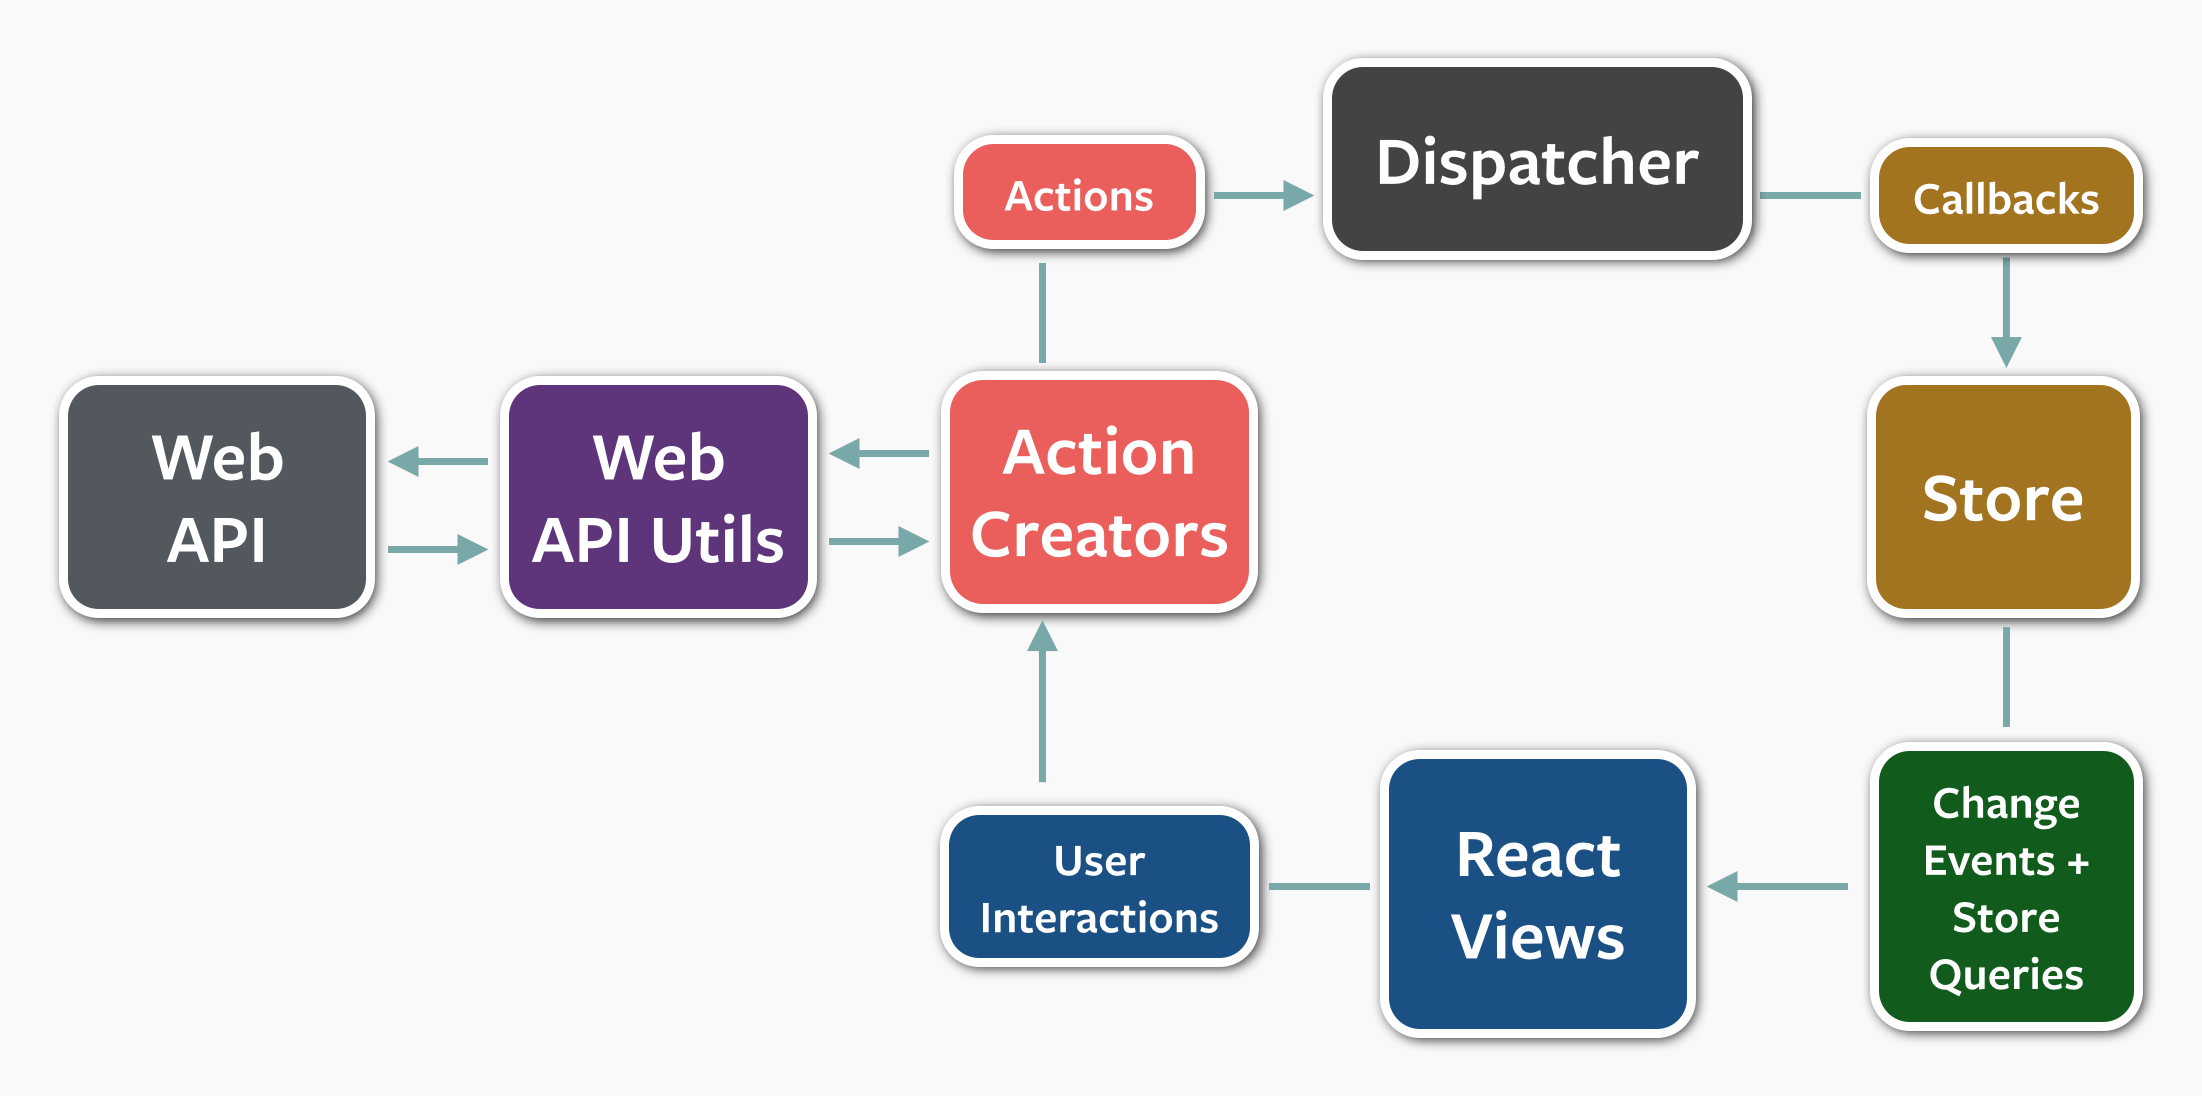
\includegraphics{./tex2pdf.11982/f036eec1d3c2a11ed0dc84a745047c5dd18c1c54.png}
\caption{Full Flux-architecture incl. networking (source:
\url{https://facebook.github.io/react/img/blog/flux-diagram.png}
(accessed 2017-02-21))}\label{fig:flux_full}
}
\end{figure}

\hypertarget{sec:redux}{%
\subsection{Redux}\label{sec:redux}}

\begin{figure}
\hypertarget{fig:redux}{%
\centering
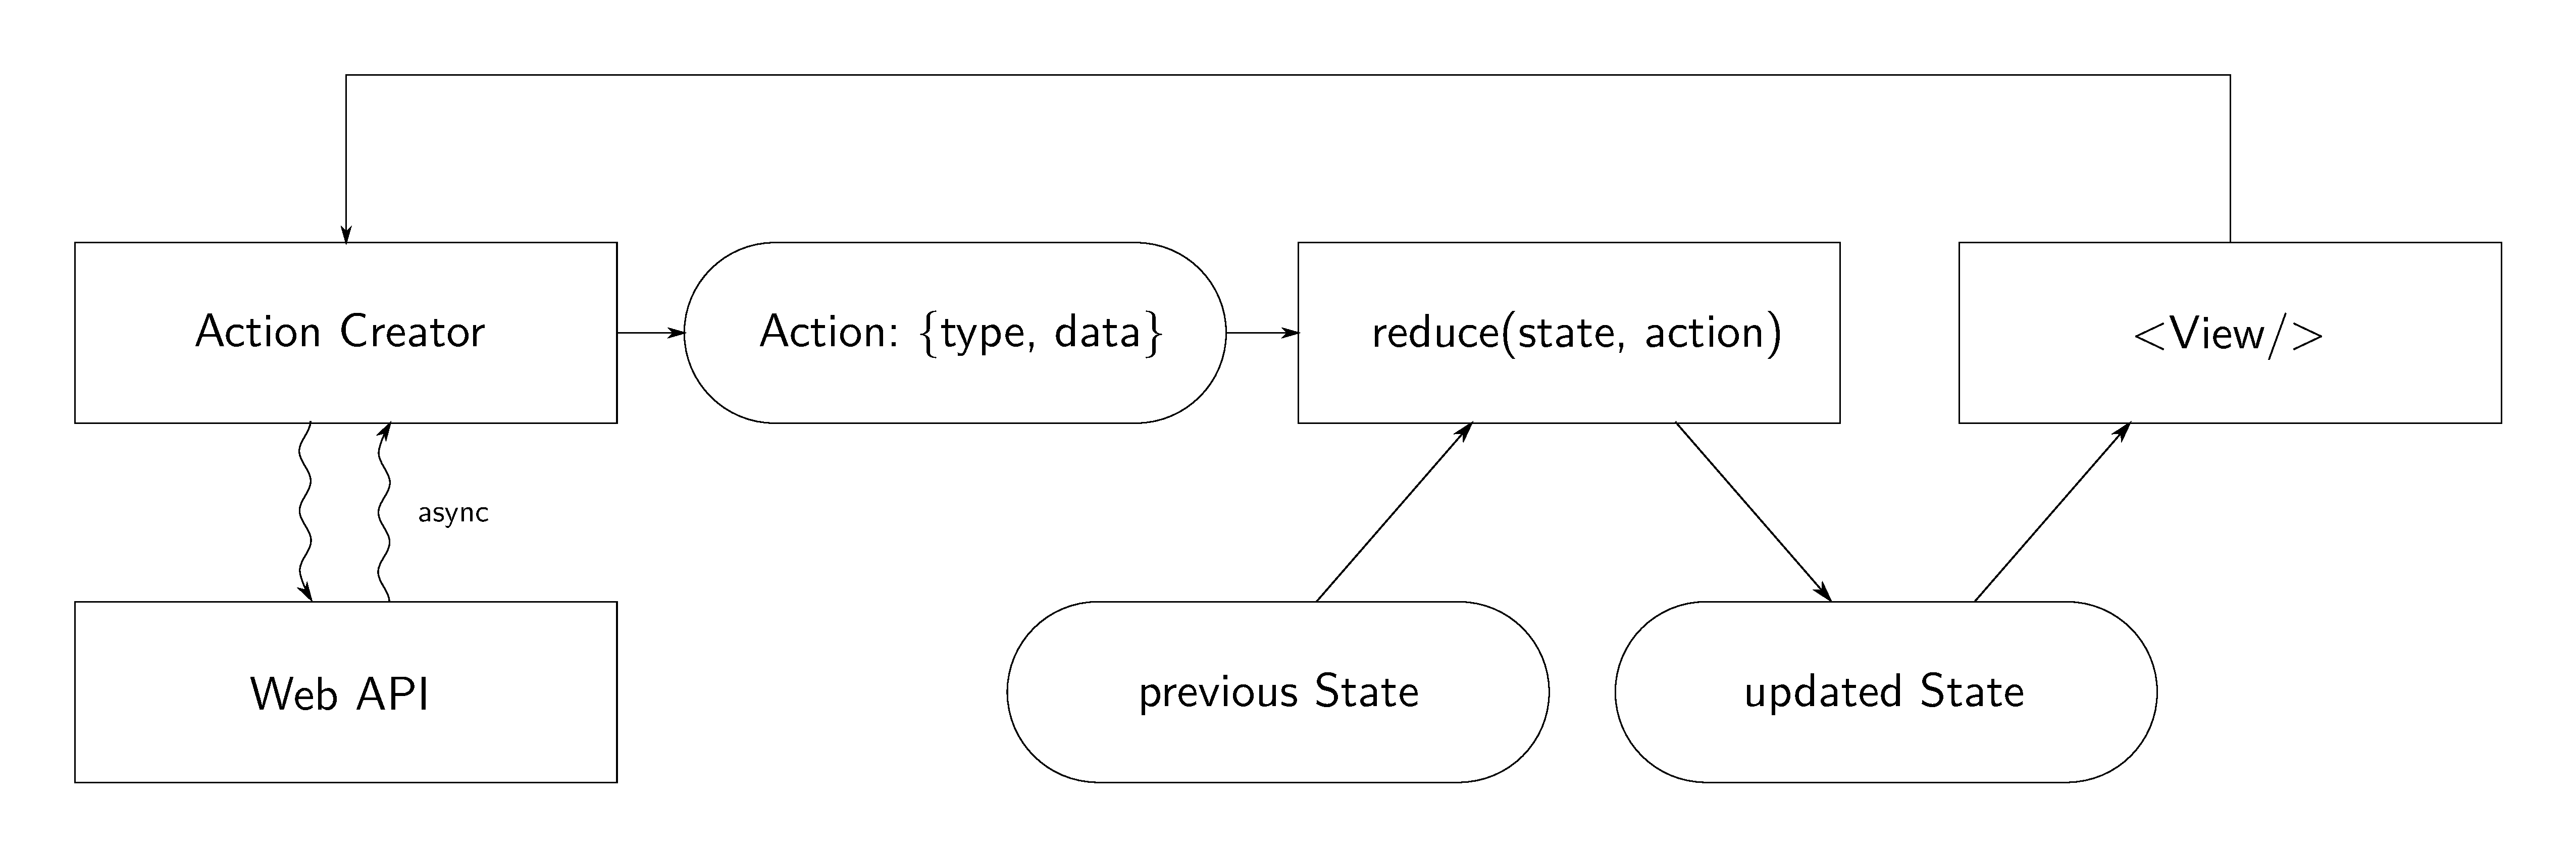
\includegraphics{./tex2pdf.11982/fbb34679c91fab49f2e56b3dc5b44cbbff8e99ee.pdf}
\caption{The redux-architecture}\label{fig:redux}
}
\end{figure}

The developers/designers of Redux list the object-oriented Flux- (see
above) and functional Elm-architecture (see below) as prior art (see
ref. ``Prior Art - Redux'' \protect\hyperlink{ref-PriorArtRedux}{n.d.}).
Redux mainly differs from Flux in eschewing the set of stateful stores,
for the Elm-like solution of having a single object as app-state, that a
single reducer-function
\passthrough{\lstinline!(state, action) => state'!} gets applied to for
every new action, thus updating the state (see fig.~\ref{fig:redux}). As
such there formally is also no need for a dispatcher, as there is only a
single function updating the state. However, in praxis usually a very
thin utility library is used, that manages state and reducers and
provides a \passthrough{\lstinline!dispatch!}-function with which the
reduction can be triggered. Separation of concerns -- achieved in Flux
via its larger number of stores -- can be achieved in Redux by having
the reducer function call other functions, e.g.~one per subobject/-tree
of the state.

As the simplest implementation of this architecture consists of only a
single function and a component that feeds actions into it, the learning
curve is relatively flat compared to Flux and almost flat compared to
Angular's MVC.

Redux profits from immutable data-structures for the app-state even more
than Flux. The reducer function is supposed to be stateless and
side-effect free (i.e.~pure). In this particular case this means that
parts of the system, that still hold references to the previous state,
shouldn't be influenced by the state-update. If they want the new state,
they'll get notified through their subscription. Using immutable data
guarantees this side-effect freeness to some extent; nothing can prevent
any point in the code from accessing the global
\passthrough{\lstinline!window!}-scope in JavaScript though -- however
it's very bad practice to do so and thus should universally be avoided.
This property also means that you should try to move as much busieness
logic as possible to the reducer, as it's comparatively easy to reason
about and thus debug. For all things that require side-effects
(e.g.~anything asynchronous like networking) action-creators are the
go-to solution -- same as in Flux.

\hypertarget{sec:ng-redux}{%
\subsection{Ng-Redux}\label{sec:ng-redux}}

Ng-Redux (see ref. \emph{Ng-Redux: Angular Bindings for Redux}
{[}\protect\hyperlink{ref-ngreduxAngularbindings2018}{2015}{]}
\protect\hyperlink{ref-ngreduxAngularbindings2018}{2018}) is a framework
that is based on the Redux-architecture and is designed to be used with
Angular applications. The latter handles the Components/Directives and
their updates of the DOM, whereas Ng-Redux manages the application
state. In this combination, the frameworks binds functions to the
angular controllers to trigger any of the available actions. Even more
importantly, it allows registering a
\passthrough{\lstinline!selectFromState!}-function that gets run after
the app-state has been updated and the result of which is then bound to
the controller. Ng-Redux also provides a middleware-system for plugins
that can modify actions and state before and after a reduction step and
can trigger side-effects. For example \enquote{thunk} provides a
convenient way to handle asynchronicity in reducers, by passing a
dispatch-function to them that they can call at any later point in time
(e.g.~when an HTTP request returns). Another example is the
\passthrough{\lstinline!ngUiRouterMiddleware!} that allows interfacing
with browsers' history-API (and thus URL in the URL-bar). That
middleware also conveniently adds this information (e.g.~current route
and route-parameters) to the application state, where components can
retrieve them like any other part of the state.

\hypertarget{sec:elm-architecture}{%
\subsection{Elm-Architecture}\label{sec:elm-architecture}}

Elm (see ref. ``Elm Language''
\protect\hyperlink{ref-ElmLanguage}{n.d.}) is a functional language
whose designers set out to create something as accessible to newcomers
as Python or Javascript. It can be used to build front-end web
applications. The original Elm-architecture was based on functional
reactive programming -- i.e.~using streams/observables like CycleJS' MVI
(see below) that it inspired as well -- but they have since been removed
to make it more accessible to newcomers. The current architecture (see
ref. ``The Elm Architecture · an Introduction to Elm''
\protect\hyperlink{ref-ElmArchitectureIntroduction}{n.d.}), in its basic
form, requires one to define the following three functions and then, in
the main function, pass these three to one of several startup functions
(e.g. \passthrough{\lstinline!Html.beginnerProgram!}):

\begin{itemize}
\tightlist
\item
  \passthrough{\lstinline!model : Model!}, that initializes the
  app-state.
\item
  \passthrough{\lstinline!update : Msg -> Model -> Model!} is a function
  that takes a \passthrough{\lstinline!Msg!} and a
  \passthrough{\lstinline!Model!} and returns an (updated)
  \passthrough{\lstinline!Model!}. This function performs the same role
  as \passthrough{\lstinline!reduce!} in Redux, with
  \passthrough{\lstinline!Msg!}s in Elm being the equivalent to actions
  in Redux.
\item
  And lastly, \passthrough{\lstinline!view : Model -> Html Msg!} to
  produce the HTML from the model. In Redux a library like react or, as
  is the case of the work at hand, angular would be used to do this
  rendering of \passthrough{\lstinline!Model!} to HTML.
\end{itemize}

As Elm is a pure (i.e.~side-effect free) language, these can't handle
asynchronity yet (e.g.~HTTP-requests, websockets) or even just produce
random numbers. The full architecture, that handles these side-effects,
looks as follows (and is run via
\passthrough{\lstinline!Html.program!}):

\begin{itemize}
\tightlist
\item
  \passthrough{\lstinline!init : (Model, Cmd Msg)!} fulfills the same
  role as \passthrough{\lstinline!model!}, but also defines the first
  \passthrough{\lstinline!Cmd!}. These commands allow \emph{requesting}
  for side-effectful computations like asynchronous operations
  (e.g.~HTTP-requests) or random number generation. The result of the
  \passthrough{\lstinline!Cmd!} is fed back as
  \passthrough{\lstinline!Msg!} to the next
  \passthrough{\lstinline!update!}.
\item
  the function
  \passthrough{\lstinline!update : Msg -> Model -> (Model, Cmd Msg)!},
  in this variant of the architecture, also returns a
  \passthrough{\lstinline!Cmd!} to allow triggering messages
  (\enquote{actions} in redux-terms) depending on user input or the
  results of previous \passthrough{\lstinline!Cmd!}s. This allows
  keeping all of the business-logic in the
  \passthrough{\lstinline!update!}-function (as compared to Flux'/Redux'
  action-creators) but trades off the quality, that every user-input or
  websocket message can only trigger exactly one action and thus exactly
  one update (thus making endless-loops possible again) 
\item
  \passthrough{\lstinline!subscriptions : Model -> Sub Msg!} allows to
  set up additional sources for \passthrough{\lstinline!Msg!}s beside
  user-input, things that \emph{push}, e.g.~listening on a websocket.
\item
  \passthrough{\lstinline!view : Model -> Html Msg!} works the same as
  in the simple variant.
\end{itemize}

\hypertarget{cyclejs-mvi}{%
\subsection{CycleJS MVI}\label{cyclejs-mvi}}

CycleJS is a framework based on \enquote{functional reactive
programming} (short FRP). The framework's is following a
Model-View-Intent architecture that is similar to the Redux- and
(original) Elm-architectures.

As an FRP-based framework, it uses observables/streams of messages for
its internal data-flows. These can be thought of as as Promises that can
trigger multiple times, or even more abstract, as pipes that manipulate
data flowing through. These observables/streams can be composed to form
a larger system. The integral part developer's using the framework need
to specify is a function
\passthrough{\lstinline!main(sources) => (\{ DOM: htmlStream\})!} (see
fig.~\ref{fig:cyclejs}) that takes a driver
\enquote{\passthrough{\lstinline!sources!}} like the DOM-driver that
allows creating stream-sources (e.g.~click events on a button). One
would then apply any data-manipulations in the function and return a
stream of virtual DOM. In the very simple code-example given below, for
every input-event a piece of data/a message would travel down the
chained functions and end up as a virtual DOM object. This
\passthrough{\lstinline!main!}-function is passed to the
\passthrough{\lstinline!run!}-function to start the app. A simple
\enquote{hello world}-application for CycleJS could look like the
following:

\begin{lstlisting}[caption={Example CycleJS app}, label=fig:cyclejs]
import {run} from '@cycle/xstream-run';
import {div, label, input, hr, h1, makeDOMDriver} from '@cycle/dom';

function main(sources) {
  const sinks = {
    DOM: sources.DOM.select('.field').events('input')
      .map(ev => ev.target.value) // get text from field
      .startWith('') // initial value / first stream-message
      .map(name =>
        div([
          label('Name:'),
          input('.field', {attrs: {type: 'text'}}),
          hr(),
          h1('Hello ' + name),
        ])
      )
  };
  return sinks;
}

run(main, { DOM: makeDOMDriver('#app-container') });
\end{lstlisting}

For more complex applications, an architecture similar to Redux/Elm,
called \enquote{Model-View-Intent} is recommended. For this, the stream
in \passthrough{\lstinline!main!} is split into three consecutive
sections:

\begin{itemize}
\tightlist
\item
  \textbf{Intent}-functions that set up the input streams from
  event-sources (e.g.~DOM and websockets) and return \enquote{intents}
  that are equivalent to Flux'/Redux' actions and Elm's messages.
\item
  The \textbf{model}-stage is usually implemented as a function that is
  \passthrough{\lstinline!reduce!}'d over the model (equivalent to how
  Redux deals with state-updates)
\item
  And lastly the \textbf{view}-stage takes the entire model and produces
  VDOM-messages.
\end{itemize}

Separation of concerns happens by using sub-functions or splitting the
stream at each stage (or starting with several sources at the
intent-stage) and combining them at the end of that respective stage.
Thus at the boundary between each of the three stages all streams are
unified into one stream that is connected to the next stage.

\hypertarget{state-of-the-art-summary}{%
\section{State-of-the Art Summary}\label{state-of-the-art-summary}}

\hypertarget{sec:methodology}{%
\chapter{Methodology}\label{sec:methodology}}

\hypertarget{design-science-in-information-systems-research}{%
\section{Design Science in Information Systems
Research}\label{design-science-in-information-systems-research}}

For the work at hand the methodological framework presented in
\enquote{Design Science in Information Systems Research} by Hevner et
al. (\protect\hyperlink{ref-HevnerDesignScienceInformation2004}{2004})
was used. This section aims to give a short overview over it, while the
next one sec.~\ref{sec:suggested-solution} will address them for this
thesis work.

\hypertarget{design-science}{%
\subsection{Design Science}\label{design-science}}

Hevner et al state that a lot of the research surrounding information
systems can be described as design- and/or behavioral science.

It roughly defines \textbf{behavioral science} with regard to
IS-research as concerned with the analysis of the interactions of people
and technology, with the goal of uncovering \enquote{truths} and
predicting or explaining phenomena surrounding these interactions.

In comparison, Hevner et al describe \textbf{design science} as
concerned with problem solving and construction with the background that
doing so leads to understanding the addressed \enquote{wicked} problem
(see section \ref{sec:wicked}). It diffentiates itself from
\textbf{routine design} by addressing problems without existing
best-practices/requisite knowledge and solves them unique/innovative
ways, or improves efficiency. By doing so, new knowledge is contributed
to the foundations and methodolgies. Design-science usually also
produces prototypes instead of full-grown systems.

The paper presents \textbf{two fundamental questions} of design research
as \enquote{What utility does the new artifact provide?} and
\enquote{What demonstrates that utility?}.

\hypertarget{sec:wicked}{%
\subsection{Wicked Problems}\label{sec:wicked}}

Hevner et al define \enquote{wicked} problems as those with
\enquote{unstable requirements, ill-defined environmental contexts,
complex interactions among subcomponents of problem and solution, an
inherent flexibility to change design processes and artifacts and a
critical dependence on human cognitive abilities (e.g.~creativity) and
social abilities (e.g.~teamwork) for effective solutions}. The term was
first used by Churchman
(\protect\hyperlink{ref-ChurchmanGuesteditorialWicked1967a}{1967}) and
defined by Rittel and Webber
(\protect\hyperlink{ref-RittelDilemmasgeneraltheory1973}{1973}) (with a
set of criteria that are somewhat different in detail). Hevner et al
cite also cite Brooks
(\protect\hyperlink{ref-BrooksNoSilverBullet1987}{1987}) and
(\protect\hyperlink{ref-BrooksComputerScientistToolsmith1996}{1996}).

\hypertarget{sec:des-proc-and-artifacts}{%
\subsection{Design Processes and
Artifacts}\label{sec:des-proc-and-artifacts}}

March and Smith
(\protect\hyperlink{ref-MarchDesignnaturalscience1995}{1995}) list two
processes involved in design, \textbf{build/generate} and
\textbf{evaluate}, that form a cycle (see fig.~\ref{fig:hevner}). They
differentiate the artifacts produced as:

\begin{itemize}
\tightlist
\item
  \textbf{constructs} that provide the language to define problems and
  solutions (e.g.~programming languages)
\item
  \textbf{models} that abstract and represent these and allow exploring
  the effects of design decisions
\item
  \textbf{methods} that define how to solve problems or aid with
  searching the problem-space (e.g.~algorithms, best practices)
\item
  \textbf{instantiations} that demonstrate feasibility and enable
  assessing suitability for the intended purpose
\end{itemize}

\hypertarget{design-science-research-guidelines}{%
\subsection{Design-Science Research
Guidelines}\label{design-science-research-guidelines}}

\begin{figure}
\hypertarget{fig:hevner}{%
\centering
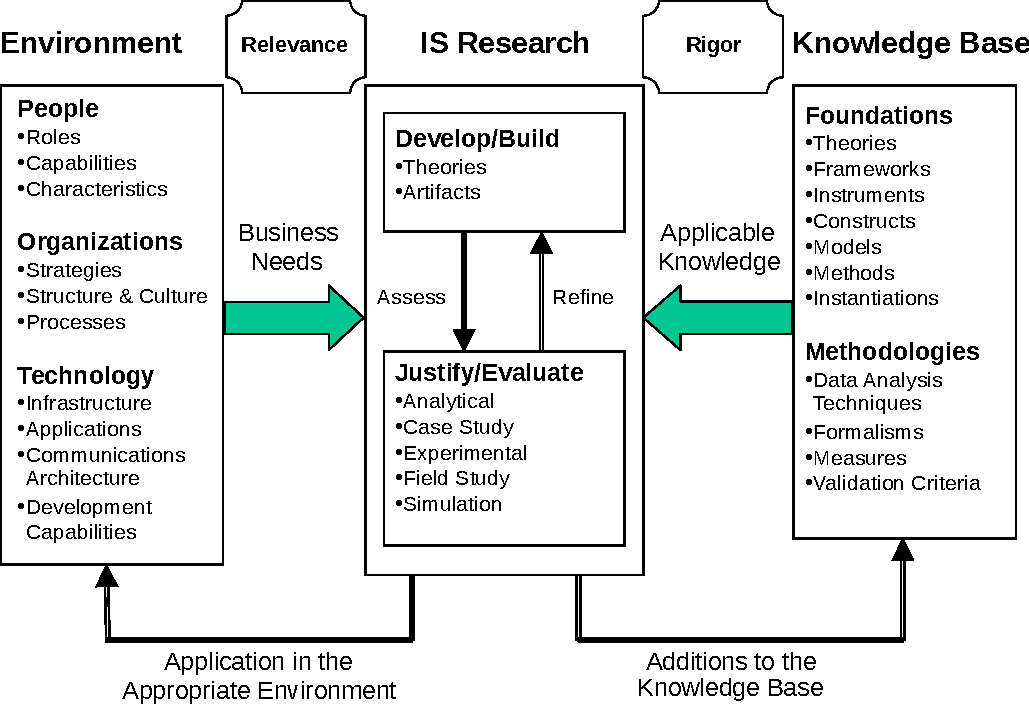
\includegraphics{./tex2pdf.11982/0e279f260acba9d3b2d9a4874e160018fa2df799.pdf}
\caption{Information Systems Research Framework (Hevner et al.
\protect\hyperlink{ref-HevnerDesignScienceInformation2004}{2004})}\label{fig:hevner}
}
\end{figure}

Hevner et al.
(\protect\hyperlink{ref-HevnerDesignScienceInformation2004}{2004})
defines seven guidelines that design-science in information systems
should address (but not necessarily come-what-may adhere to). Section
\ref{sec:suggested-solution} will address them for the work at hand.

They are as follows:

\begin{itemize}
\tightlist
\item
  \textbf{Design as an Artifact.} \enquote{Design-science research must
  produce a viable artifact in the form of a construct, a model, a
  method, or an instantiation.} This allows demonstrating feasibility --
  for cases where that wasn't a given yet -- thus making it research (as
  opposed to routine design). 
\item
  \textbf{Problem Relevance.} \enquote{The objective of design-science
  research is to develop technology-based solutions to important and
  relevant business problems.} Relevancy here is with respect to a
  \enquote{constituent community} (e.g.~IS practitioners)
\item
  \textbf{Design Evaluation.} \enquote{The utility, quality, and
  efficacy of a design artifact must be rigorously demonstrated via
  well-executed evaluation methods.} This usually requires integration
  into the usage context (to see if it \enquote{works} there or is
  \enquote{good} in it), the definition of appropriate metrics and
  gathering of appropriate data. Evaluation provides valuable and
  necessary feedback for the design iterations (see
  fig.~\ref{fig:hevner})
\item
  \textbf{Research Contributions.} \enquote{Effective design-science
  research must provide clear and verifiable contributions in the areas
  of the design artifact, design foundations, and/or design
  methodologies.} Important here is the novelty of the artifact -- by
  extending or innovatively (re-)applying previous knowledge -- as well
  as its generality and significance.
\item
  \textbf{Research Rigor.} \enquote{Design-science research relies upon
  the application of rigorous methods in both the construction and
  evaluation of the design artifact.} This means applying existing
  foundations and methodologies, using effective metrics and
  formalizing. Note, however, that an overemphasis on rigor can often
  lead to lower relevance (Lee
  \protect\hyperlink{ref-LeeInauguralEditorComments1999}{1999}), as many
  environments and artifacts defy an excessive formalism (see
  \enquote{wicked problems} in section \ref{sec:wicked}).
\item
  \textbf{Design as a Search Process.} \enquote{The search for an
  effective artifact requires utilizing available means to reach desired
  ends while satisfying laws in the problem environment.} This entails
  using heuristic search stragegies (e.g.~best-practices as starting
  point) in the generate/test-cycle (see fig.~\ref{fig:hevner}).
  However, again, it might not be possible to formalize or even
  determine any of these, due to the \enquote{wicked} (see section
  \ref{sec:wicked}) nature of tackled problems. As a result it might
  often be necessary to only work on simpler sub-problems, giving up
  relevancy in turn.
\item
  \textbf{Communication of Research} \enquote{Design-science research
  must be presented effectively both to technology-oriented as well as
  management-oriented audiences.} For the former the construction and
  evaluation process are important (e.g.~to allow reproduction). For the
  latter the question boils down to \enquote{Is it worth the effort to
  use the artifact for my business?}. This can be broken down as
  \enquote{What knowledge is required?} respectively \enquote{Who can
  use it?}, \enquote{How imporant is the problem?}, \enquote{How
  effective is the solution?} as well as some details in appendices to
  appreciating the work.
\end{itemize}

\hypertarget{design-evaluation-methods}{%
\subsection{Design Evaluation Methods}\label{design-evaluation-methods}}

Observational methods:

\begin{itemize}
\tightlist
\item
  \textbf{Case Study} \enquote{Study artifact in depth in business
  environment} 
\item
  \textbf{Field Study} \enquote{Monitor use of artifact in multiple
  projects} 
\end{itemize}

Analytical methods:

\begin{itemize}
\tightlist
\item
  \textbf{Static Analysis} \enquote{Examine structure of artifact for
  static qualities (e.g., complexity)} 
\item
  \textbf{Architecture Analysis} \enquote{Study fit of artifact into
  technical IS architecture} 
\item
  \textbf{Optimization} \enquote{Demonstrate inherent optimal properties
  of artifact or provide optimality bounds on artifact behavior}
\item
  \textbf{Dynamic Analysis} \enquote{Study artifact in use for dynamic
  qualities (e.g., performance)}
\end{itemize}

Experimental Methods:

\begin{itemize}
\tightlist
\item
  \textbf{Controlled Experiment} \enquote{Study artifact in controlled
  environment for qualities (e.g., usability)}
\item
  \textbf{Simulation} \enquote{Execute artifact with artificial data}
\end{itemize}

Testing:

\begin{itemize}
\tightlist
\item
  \textbf{Functional (Black Box) Testing} \enquote{Execute artifact
  interfaces to discover failures and identify defects}
\item
  \textbf{Structural (White Box) Testing} \enquote{Perform coverage
  testing of some metric (e.g., execution paths) in the artifact
  implementation}
\end{itemize}

Descriptive Methods:

\begin{itemize}
\tightlist
\item
  \textbf{Informed Argument} \enquote{Use information from the knowledge
  base (e.g., relevant research) to build a convincing argument for the
  artifact's utility} 
\item
  \textbf{Scenarios} \enquote{Construct detailed scenarios around the
  artifact to demonstrate its utility}
\end{itemize}

\hypertarget{sec:suggested-solution}{%
\chapter{Suggested Solution}\label{sec:suggested-solution}}

As already mentioned in the problem description (chapter
\ref{sec:probdescr}), the rework and restructuring started with a
codebase using Angular (see section \ref{sec:angular-mvc}), all modules
included one-by-one in the \passthrough{\lstinline!index.jsp!}, and some
bootstrap-theme (see section \ref{sec:bootstrap}) for styling. Bugs were
hard to solve due to the \enquote{grown} code-base and the somewhat
ambiguous architecture stemming both the wide range of concepts in
angular that required understanding and best-practices as well as our
grasp of them. Additionally, the visual style was neither polished nor
projecting a unique identity.

As part of a research-project together with our partner Meinkauf, the
Researchstudio Smart Agent Technologies was tasked with developing a
platform-independent mobile application and used Ionic (see ref. Ionic
\protect\hyperlink{ref-IonicIonicFramework}{n.d.}), i.e.~a tooling
default, that at the time consisted of Phonegap (see ref. ``PhoneGap''
\protect\hyperlink{ref-PhoneGap}{n.d.}), Angular 1.x, SCSS (see section
\ref{sec:scss}), ionic-specific CSS and its own command-line-tool. This
project presented a good opportunity to try out a different
architecture, to deal with the ambiguities and maintenance problems we
were experiencing with the Web of Needs owner-application.

\hypertarget{sec:technology-stack}{%
\section{Technology Stack}\label{sec:technology-stack}}

\hypertarget{sec:research-rigor}{%
\section{Research Rigor}\label{sec:research-rigor}}

\enquote{Design-science research relies upon the application of rigorous
methods in both the construction and evaluation of the design artifact.}

\hypertarget{sec:process}{%
\section{Process}\label{sec:process}}

\hypertarget{sec:architecture}{%
\section{Architecture}\label{sec:architecture}}

We're using a variation of the redux-architecture (see sections
\ref{sec:redux} and \ref{sec:ng-redux} respectively) for the
won-owner-webapp JavaScript-client.

This section will document in what ways our architecture diverges from
or builds on top of basic redux, as well as list experiences and
style-recommendations derived from using it.

\begin{figure}
\hypertarget{fig:adapted-redux}{%
\centering
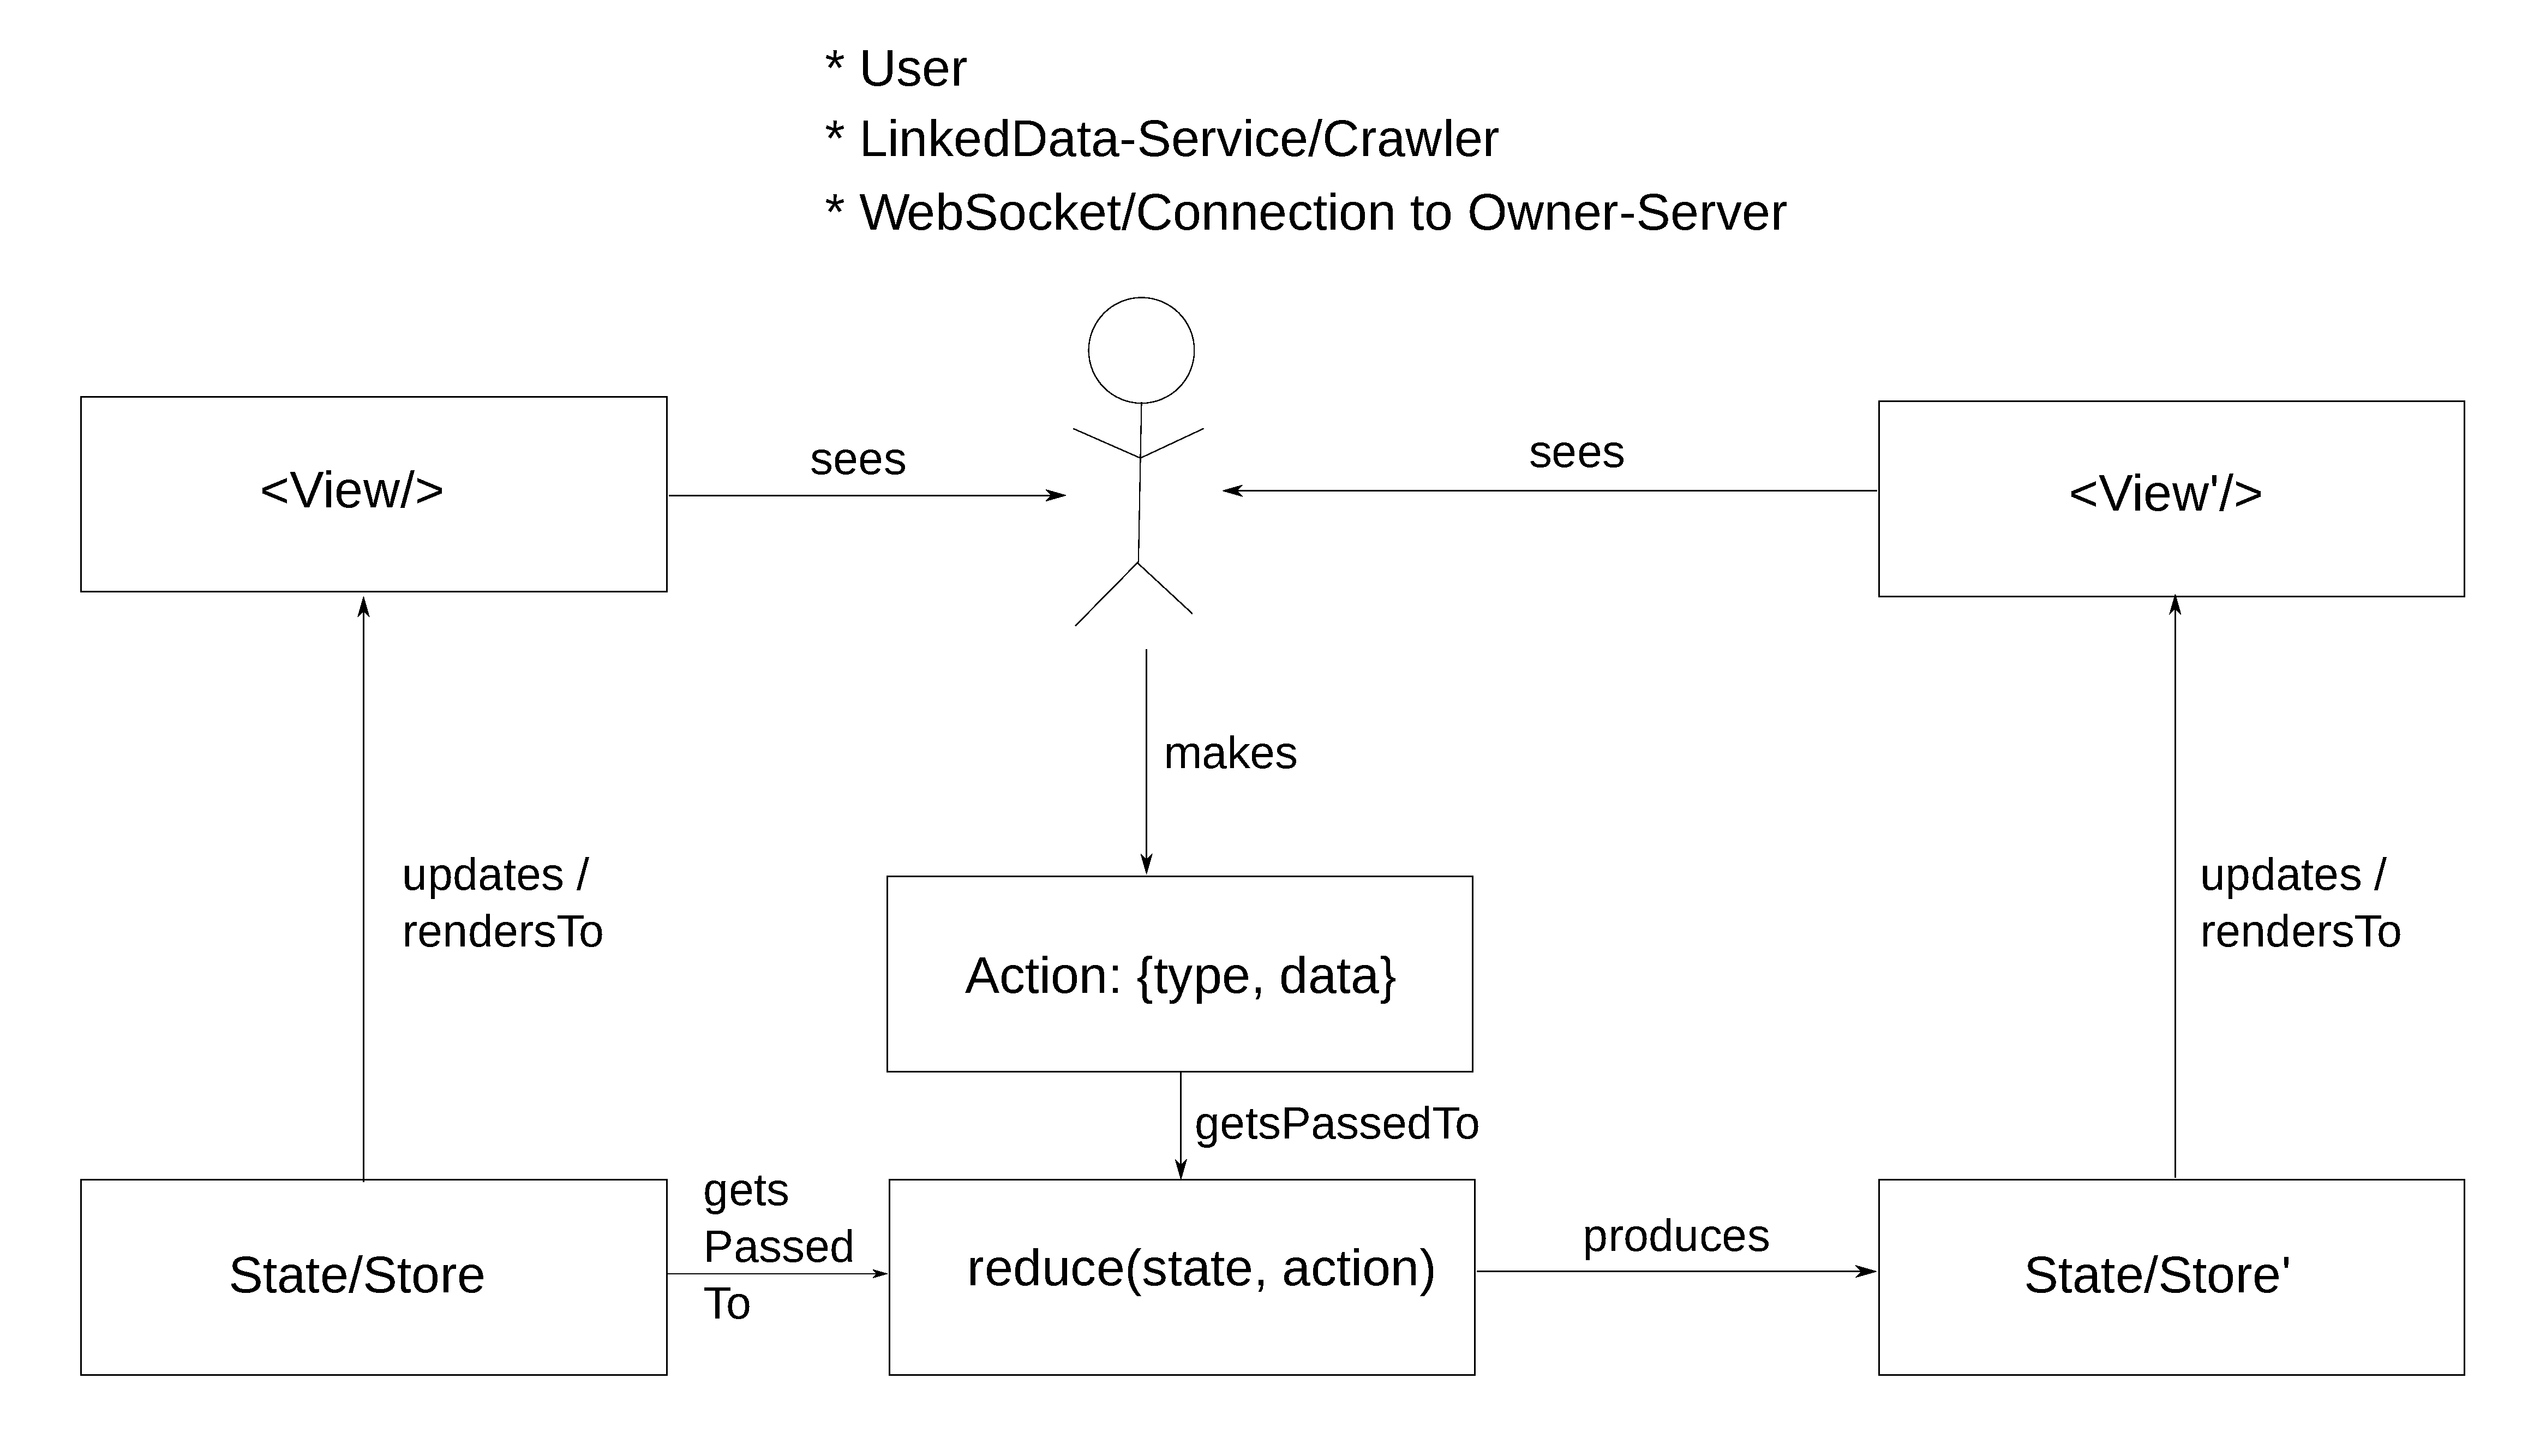
\includegraphics{./tex2pdf.11982/b93b469a783e9ff3c749a7cfca53ffdebdb5cae0.pdf}
\caption{Redux architecture in client-side
owner-app}\label{fig:adapted-redux}
}
\end{figure}

\hypertarget{sec:action-creators}{%
\subsection{Action Creators}\label{sec:action-creators}}

Can be found in \passthrough{\lstinline!app/actions/actions.js!}

Anything that can cause \textbf{side-effects} or is
\textbf{asynchronous} should happen in these (tough they can also be
synchronous -- see \passthrough{\lstinline!INJ\_DEFAULT!}) They should
only be triggered by either the user or a push from the server via the
\passthrough{\lstinline!messagingAgent.js!}. In both cases they cause a
\textbf{single}(!) action to be dispatched and thus passed as input to
the reducer-function.

All actions are declared in the
\passthrough{\lstinline!actionHierarchy!}-object in
\passthrough{\lstinline!action.js!}. From that two objects are
generated:

\begin{itemize}
\tightlist
\item
  \passthrough{\lstinline!actionTypes!}, which contains string-constants
  (e.g.
  \passthrough{\lstinline!actionTypes.drafts.change.title === 'drafts.change.title'!})
\item
  \passthrough{\lstinline!actionCreators!}, which houses the action
  creators. For the sake of injecting them with ng-redux, they are
  organised with \passthrough{\lstinline!\_\_!} as separator (e.g.
\item
  \passthrough{\lstinline!actionCreators.drafts\_\_change\_\_title('some title')!}
\end{itemize}

The easiest way to create actions without side-effects is to just place
an \passthrough{\lstinline!myAction: INJ\_DEFAULT!}. This results in an
action-creator that just dispatches all function-arguments as payload,
i.e.
\passthrough{\lstinline!actionCreators.myAction = argument => (\{type: 'myAction', payload: argument\})!}

Actions and their creators should always describe \textbf{high-level
user stories/interactions} like
\passthrough{\lstinline!matches.receivedNew!} or
\passthrough{\lstinline!publishPost!} (as opposed to something like
\passthrough{\lstinline!matches.add!} or
\passthrough{\lstinline!data.set!}) Action-creators encapsule all
sideeffectful computation, as opposed to the reducers which (within the
limits of JavaScript) are guaranteed to be side-effect-free. Thus, we
should do \textbf{as much as possible within the reducers}. This
decreases the surprise-factor, coupling and bug-proneness of our code
and increases its maintainability.

\hypertarget{sec:actions}{%
\subsection{Actions}\label{sec:actions}}

They are objects that serve as input for the reducer. Usually they
consist of a type and a payload, e.g.:

\begin{lstlisting}[caption={Example action object}, label=fig:actionjson]
{
  type: "needs.close"
  payload: {
    ownNeedUri: "https://node.matchat.org/won/resource/need/1234"
  }
}
\end{lstlisting}

These should describe high-level interactions from the user (or server
if initiated there).\\
A full list of action-types, used in the owner-application\\
can be found in \passthrough{\lstinline!app/actions/actions.js!}.

\hypertarget{sec:reducers}{%
\subsection{Reducers}\label{sec:reducers}}

Can be found in \passthrough{\lstinline!app/reducers/reducers.js!}

These are \textbf{side-effect-free}. Thus, as much of the implementation
as possible should be here instead of in the action-creators to profit
from this guarantee and steer clear of possible sources for bugs that
are hard to track down.

Usually they will consist of simple switch-case statements. A simple
reducer that would keep track of own needs could (in-part) look as
follows:

\begin{lstlisting}[caption={Simple example reducer.}, label=fig:reducer]
import { actionTypes } from '../actions/actions';
import Immutable from 'immutable';
import won from '../won-es6';

const initialState = Immutable.fromJS({
    //...
    ownNeeds: {},
});

export default function(allNeeds = initialState, action = {}) {
  switch(action.type) {
    case actionTypes.logout:
      return initialState;

    case actionTypes.needs.close:
      return allNeeds.setIn([
        "ownNeeds", action.payload.ownNeedUri, 'won:isInState'
      ], won.WON.InactiveCompacted);

    //...

    default:
      return allNeeds;
}
\end{lstlisting}

\hypertarget{sec:components}{%
\subsection{Components}\label{sec:components}}

They live in \passthrough{\lstinline!app/components/!}.

Top-level components (views in the angular-sense) have their own folders
(e.g. \passthrough{\lstinline!app/components/create-need/!} and are
split in two files). You'll need to add them to the routing (see below)
to be able to switch the routing-state to these.

Non-top-level components are implemented as directives. A very simple
demo-component, that would render the title and description of a need to
the DOM-tree and allow closing it (i.e.~making it unreachable to contact
requests) via a click on \enquote{{[}CLOSE{]}}, would look as follows:

\begin{lstlisting}[caption={Example component.}, label=fig:example-component]
import angular from 'angular';
import 'ng-redux';
import { actionCreators }  from '../actions/actions';
import { attach } from '../utils.js'
import { seeksOrIs, connect2Redux } from '../won-utils'

// angular utilities required to integrate the component
// into the redux architecture via the `connect2Redux`-
// function.
const serviceDependencies = ['$ngRedux', '$scope'];

// factory function for the directive:
function genComponentConf() {

  const template = `
    <h1>{{ self.needContent.get('dc:title') }} [DEMO]</h1>
    <p>{{ self.needContent.get('won:hasTextDescription') }}</p>
    <a ng-click="self.needs__close(self.need.get('@id'))">
        [CLOSE]
    </a>
  `;

  class Controller {
    constructor() {

      // does `controller.<serviceName> = <serviceName>`
      // for all services injected via `arguments`
      attach(this, serviceDependencies, arguments);

      const selectFromState = (state) => {
        const need =
          state.getIn(['needs', 'ownNeeds', this.needUri]);

        // need and needContent will be bound to the
        // controller (=scope) and thus be available
        // in the template.
        return {
          need,
          needContent: need && seeksOrIs(need),
        }
      };
      connect2Redux(
        selectFromState, // result will be bound to `this`
        actionCreators, // will be bound to `this`
        ['self.needUri'], // component property used in select
        this // the controller
      );
    }
  }
  Controller.$inject = serviceDependencies;

  // directive configuration:
  return {
    scope: { needUri: '=' }, // available property on HTML-tag

    controller: Controller,
    template: template

    restrict: 'E', // directive only usable as HTML-tag
    controllerAs: 'self', //ctrl available via `self` in template
    bindToController: true, //ctrl is scope for template
  }
}

export default angular.module(
  'won.owner.components.demoComponent',
  [ /* here: any dependencies using angular */ ]
)
.directive('wonDemoComponent', genComponentConf)
.name
// ^ exported name used by importing component in dependency-array
\end{lstlisting}

The component can then be used by a \textbf{parent component} via:

\begin{lstlisting}[caption={Usage in parent component.}, label=fig:usage-in-parent-component]
// ...

import demoComponentName from './demo-component.js'

// ...

function genComponentConf() {
  const template = `
    <h1>All Owned Needs</h1>
    <won-demo-component
      ng-repeat="uri in self.needUris"
      needUri="uri">
    </won-demo-component>`

  //...
}

export default angular.module(
  'won.owner.components.demoParent',

  // so angular knows to run the child first:
  [ demoComponentName ]
)
.directive('wonDemoParent', genComponentConf)
.name
\end{lstlisting}

As you can see, there is quite a bit boiler-plate required by angular.
All that is required by (ng-)redux is the listener to the state set up
by \passthrough{\lstinline!connect2Redux!}.

Among the boiler-plate there is a few details I'd like to point out,
that make working with Angular 1.X a lot less painful. I'll go through
it top-to-bottom.

The \passthrough{\lstinline!serviceDependencies!} lists the angular
services, that will be passed to the constructor of the directive.
Assigning that array with the dependency-names to the Controller class
via \passthrough{\lstinline!$inject!} makes sure Angular does just that,
even if the code is minified. Per default angular reads the names of the
arguments of the constructor, but during minification that information
is lost. By setting \passthrough{\lstinline!strictDi: true!} when
starting up angular in \passthrough{\lstinline!app/app\_jspm.js!} we
make sure angular complains if the injection array isn't there. The
\passthrough{\lstinline!attach!}-function then takes the constructor's
arguments (i.e.~the injected service dependencies) and assigns them as
properties to the controller-object.

The template strings (\passthrough{\lstinline!const template = '...'!})
describe the HTML that the user gets to see. When a component is first
rendered, angular parses the string and generates the required HTML,
starts up any required child-components and directives, and evaluates
any expressions in double curly braces and then replaces them with the
result of that respective expression. E.g.
\passthrough{\lstinline!<h1>\{\{ self.needContent.get('dc:title') \}\} [DEMO]</h1>!}
might become
\passthrough{\lstinline!<h1>Couch to give away [DEMO]<h1>!}. It also
makes sure that whenever these expressions change, the DOM is updated.
To do this it sets up a so called \enquote{watch} per expression. Every
time a \passthrough{\lstinline!$digest!}-cycle is triggered, all
watch-expressions are evaluated and necessary changes to the DOM made
one at a time (this is also what makes Angular 1.x terribly imperformant
compared to virtual-DOM frameworks like React and the Elm-runtime, that
batch updates). \passthrough{\lstinline!$ngRedux!} makes sure a
\passthrough{\lstinline!$digest!}-cycle is triggered every time the
redux state has been updated. Managing these
\passthrough{\lstinline!$digest!}-cycle can be a bit of a hassle at
times and the occasional source of a hard-to-track-down bug.

Also, in the template, the
\passthrough{\lstinline!ng-click="self.needs\_\_close(self.need.get('@id'))"!}
sets up a listener for a click event on the element, that executes the
code in the double quotes, in this case it calls the action-creator
\passthrough{\lstinline!needs\_\_close!} with a specific need-uri, that
makes an HTTP-request to the server and on success creates an
action-object and dispatches it, thus triggering a state-update.

Ng-redux provides us with the utility function
\passthrough{\lstinline!$ngRedux.connect(selectFromState, actionCreators)(controller)!}
that \passthrough{\lstinline!connect2Redux!} uses internally. What it
does is to set up a listener on the state managed by ng-redux. Every
time the state is updated, \passthrough{\lstinline!selectFromState!} is
run on it. Its return object is then assigned property-by-property to
the \passthrough{\lstinline!controller!}. As a convenience-feature, the
functions in \passthrough{\lstinline!actionCreators!} are wrapped with a
call to \passthrough{\lstinline!$ngRedux.dispatch!} and also get
assigned to the \passthrough{\lstinline!controller!} when the component
is initialized. Otherwise it would be necessary to write
\passthrough{\lstinline!self.$ngRedux.dispatch(self.someAction(...))!}
everywhere in the component that the action is triggered.

Note, that \passthrough{\lstinline!selectFromState!} can be used to
transform the data, that should be stored in a normalized,
redundancy-free fashion in the state, into something that is easier to
consume in the state. Frequently used selection-functions can be found
in \passthrough{\lstinline!app/selectors.js!}. Many of these use
\href{https://github.com/reactjs/reselect}{reselect} that allows caching
the results of computations until their dependencies change. This way,
if e.g.~the list of connections with their related needs and events is
needed by multiple components on the screen, the filter and group
operations are only run once (instead of once per component selecting
that data).

As a secondary function, \passthrough{\lstinline!connect2Redux!} also
unregisters any listeners and watches when the component is removed.

Some hard lessons went into using the following in the directive
configuration:

\passthrough{\lstinline!\{.js fig:directive-config caption="Essential directive configuration boilerplate."\} \{   scope: \{ \},   //...   restrict: 'E',   bindToController: true,   controllerAs: 'self', \}!}

Of these the first is the most important. It allows specifying custom
properties for the component. However, even when there are no
properties, one should always specify an (empty) scope object. This
\enquote{isolates} the scope in angular-terms. Without it, when a
property is requested (e.g.~in the template) and it's not found on the
directive itself, angular will continue to look for the property in the
scope of the enclosing directive or view. Not only that it will read
data from there, when variables are assigned, it will also write
there(!). Thus, when you assign to a variable that reads the same, as a
parent component's, you'll change the value there as well, causing
(almost certainly unintended) consequences there.

The \passthrough{\lstinline!restrict!} ensures that the directive is
only used as HTML-tag. Usually it would also be usable as
HTML-tag-property or even class. Unless you're doing something along the
lines of \passthrough{\lstinline!ng-click!} (that sets up click-handlers
on an arbitrary HTML-tag) I wouldn't recommend using the property and
definitely would always advise against using directives via class names.
Neither of these is suited well for having inner HTML.

Of the other options \passthrough{\lstinline!bindToController!} ensures
that the controller is used as scope, thus avoiding juggling two
JavaScript-objects and wondering on which the data is.
\passthrough{\lstinline!controllerAs!} binds exposes the controller to
the template as \passthrough{\lstinline!'self'!} (in this case).

\hypertarget{sec:routing}{%
\subsection{Routing}\label{sec:routing}}

We use ui-router (see ref. \emph{Ui-Router}
\protect\hyperlink{ref-uirouter}{n.d.}) and in particular the
redux-wrapper (see ref. Fenton
\protect\hyperlink{ref-FentonreduxuirouterngReduxbindings}{n.d.}) for
it.

Routing(-states, aka URLs) are configured in
\passthrough{\lstinline!configRouting.js!}. State changes are triggered
via the asynchronous action creator
\passthrough{\lstinline!actionCreators.router\_\_stateGo(stateName)!}.
The current routing-state and -parameters can be found in our app-state:

\passthrough{\lstinline!\{.js fig:routing-params-in-state caption="Routing parameters in redux state."\} $ngRedux.getState().get('router') /* => \{   currentParams: \{...\},   currentState: \{...\},   prevParams: \{...\},   prevState: \{...\} \} */!}

Also, see: Routing and Redux (ref. ``Routing and Redux · Issue \#344 ·
Researchstudio-Sat/Webofneeds''
\protect\hyperlink{ref-RoutingReduxIssue}{n.d.})

\hypertarget{sec:server-interaction}{%
\subsection{Server-Interaction}\label{sec:server-interaction}}

For \textbf{REST}-style requests,
\passthrough{\lstinline!fetch(...).then(data => \{...dispatch(...); \})!}
is used in action-creators.

If it's \textbf{linked-data-related}, the utilities in
\passthrough{\lstinline!linkeddata-service-won.js!} are used. They do
standard HTTP(S) but make sure to cache as much as possible via the
local triplestore. However, in the future this custom caching layer can
be replaced by using HTTP2 to load the large number of
RDF-documents\footnote{ad large number of documents: when your entire
  state contains of a single contact request, you still need to load 6
  documents , in 3-5 roundtrips: your need, its connection container,
  the connection to the other person's need, its event container, the
  event, and lastly the other person's need.} in one round-trip and let
the browser-chache handle repeated requests. One advantage of the
triple-store is that it stores the RDF in its natural state and
additional data can just be \enquote{poured} into the store. Anything
e.g.~related to a need can be retrieved using a SPARQL-query. One price
here however is one of performance -- some queries performed very badly
and needed to be replaced by work-arounds -- and another price is
complexity, as the custom caching logic written to avoid unnecessary
HTTP-requests yet keep the store in synch with the node-server is a
frequent source of hard to track down bugs.

JSON-LD send is \textbf{send} to the server \textbf{via a
websocket-connection}. For this case-statments for the respective action
are added in \passthrough{\lstinline!message-reducers.js!} that adds
them to the message-queu in
\passthrough{\lstinline!state.getIn(['messages', 'enqueued'])!}. The
messaging agent picks theses up and pushes them to the websocket it
manages.

New messages are \textbf{received via the web-socket}. This allows the
server to push-notify the client. The messaging agent contains a series
of handlers for different message-types that then dispatch corresponding
actions.

\hypertarget{views-and-interactions}{%
\section{Views and Interactions}\label{views-and-interactions}}

For the sake of completeness and to illustrate the usefullness, this
section will give a very brief overview over the GUI built with this
works' architecture and tooling and how it ties into the architecture at
large. For a detailed code example of a simple component see
fig.~\ref{fig:example-component} in sec.~\ref{sec:components}.

\hypertarget{sec:tooling}{%
\section{Tooling}\label{sec:tooling}}

\hypertarget{sec:es6}{%
\subsection{ES6}\label{sec:es6}}

As mentioned in section \ref{sec:technical-requirements}, one of the
goals was to improve the quality of the code, its readability and
authoring support, especially regarding expressiveness, robustness,
conciseness and bug prevention. For this it seemed natural to start
using features from the latest JavaScript standard (at the time of
writing ES6, also known as ES2015, optionally plus experimental
features). Amongst others, this would give us access to:

\begin{itemize}
\tightlist
\item
  ES6-style variable declarations (e.g.
  \passthrough{\lstinline!const x = 2; let y = 3; y = 1;!})
\item
  Native Promises (e.g.
  \passthrough{\lstinline!asyncFn().then(x => /*...*/))!})
\item
  Async-Await (e.g. \passthrough{\lstinline!const x = await asyncFn()!}
  )
\item
  Arrow-functions (e.g. \passthrough{\lstinline!x => 2*x!})
\item
  Destructuring assignment (e.g.
  \passthrough{\lstinline!const \{ a, b \} = someObj!})
\item
  ES6-Modules (e.g.
  \passthrough{\lstinline!import \{ someFn \} from './moduleA.js!})
\item
  etc
\end{itemize}

As some of these features weren't fully supported by all browsers
cross-compilation to older JavaScript versions was necessary. Also, the
module-syntax required a bundler, that combines the JavaScript modules
into one file, that can be included via a
\passthrough{\lstinline!<script>!}-tag.

\hypertarget{es6-style-variable-declarations}{%
\subsubsection{ES6-style Variable
Declarations}\label{es6-style-variable-declarations}}

ES6 also gives us \passthrough{\lstinline!const!}-variables, that throw
errors when trying to accidentally reassigning to them, and
\passthrough{\lstinline!let!}-variables that behave like
variable-declarations in other C-style-languages would. In
contrast,\passthrough{\lstinline!var!}-declarations are always scoped to
the parent-function not the containing scope, e.g.~in an if, and can be
silently re-declared, potentially causing bugs in unsuspecting
developer's hands.

\hypertarget{promises}{%
\subsubsection{Promises}\label{promises}}

These are a fix of the so-called callback hell, i.e.~code like the
following:

\passthrough{\lstinline'\{.js fig:callback-hell caption="Callback hell."\} won.login(credentials, function(error, userInfo) \{   if(!error) \{     won.getOwnedNeedUris(function(error, needUris) \{       if(!error) \{         for(int i = 0; i < needUris.length; i++) \{           var needs = [];           won.getNeed(needUris[i], function(error, need) \{             if(!error) \{               needs.push(need);               if(needs.length === needUris.length) \{                 // all callbacks have resolved, pass the result on to redux                 dispatch(actionCreators.initialPageLoad(\{                   needs: needs,                   userInfo: userInfo,                 \}));               \}             \}             else \{               handlePageLoadError(error);             \}           \}         \}       \} else \{         handlePageLoadError(error);       \}     \})   \} else \{     handlePageLoadError(error);   \} \})'}

With promises, arrow-functions\footnote{a conciser function syntax with
  slightly different behavior regarding the
  \passthrough{\lstinline!this!}-keyword, i.e.~it doesn't rebind it to
  the local scope, making them good for use within methods of ES6-style
  classes (see refs. ``Arrow Functions''
  \protect\hyperlink{ref-Arrowfunctions}{n.d.}; and ``ECMAScript 2015
  Language Specification -- ECMA-262 6th Edition''
  \protect\hyperlink{ref-ECMAScript2015Language2015}{2015}, sec. 14.2
  Arrow Function Definitions).} and the enhanced object
literals\footnote{\passthrough{\lstinline!\{needs, userInfo\}!} as
  syntactic-sugar for
  \passthrough{\lstinline!\{needs: needs, userInfo: userInfo\}!}} this
looks like:

\begin{lstlisting}[caption={Same example but using promises}, label=fig:promise-in-use]
won.login(credentials)
.then(userInfo =>
  won.getOwnedNeedUris()
  .then(needUris =>
    Promise.all(
      needUris.map(needUri => won.getNeed(needUri))
    )
  )
  .then(needs =>
    dispatch(actionCreators.initialPageLoad({needs, userInfo}))
  )
)
.catch(error => handlePageLoadError(error))
\end{lstlisting}

This is already a lot conciser and more expressive. If error occurs at
any point the control-flow will jump to the next catch in the
promise-chain and \passthrough{\lstinline!Promise.all!} makes sure all
needs finish loading before continuing. However, notice that the later
access to \passthrough{\lstinline!userInfo!} requires nesting the
Promises again.

Before the rework, the code-base was already, occasionally using
angular's \passthrough{\lstinline!$q!} as polyfill that was providing
the same functionality in different places. However, as angular-service,
\passthrough{\lstinline!$q!} required to keep all code, even
asynchronous utility-functions, within angular-services.

\hypertarget{async-await}{%
\subsubsection{Async-Await}\label{async-await}}

While promises are a great way of managing asynchronicity in our code,
async-await, a form of syntactic sugar for promises, allows further
simplifications. The code example from above
fig.~\ref{fig:promises-in-use} looks like the following, when
async-await is used:

\passthrough{\lstinline!\{.js fig:async-await caption="Same example but using async-await"\} try \{   const userInfo = await won.login(credentials);   const needUris = await won.getOwnedNeedUris();   const needs = await Promise.all(     needUris.map(needUri => won.getNeed(needUri))   );   dispatch(actionCreators.initialPageLoad(\{needs, userInfo\})) \} catch (error) \{   handlePageLoadError(error); \}!}

As you can see, this looks somewhat conciser and saves us the nesting
caused due to the later use of \passthrough{\lstinline!userInfo!}. In
this example this is a rather small difference, but the code-base had
contained some three to five layer nesting that could be significantly
simplified using async-await.

\hypertarget{es6-modules-and-bundling}{%
\subsubsection{ES6-Modules and
Bundling}\label{es6-modules-and-bundling}}

Previously we'd been including the JS-files via
\passthrough{\lstinline!<script>!}-tags in
\passthrough{\lstinline!index.html!} which was very fragile as
dependency information wasn't solely managed by the scripts themselves
but also redundantly managed via this include list. Also, it depended
heavily on angular's dependency-injection mechanism, thus even
utility-modules had to use that or expose themselves to global scope
(and then be included in right order, lest they crash during startup). A
less standardized variant here would have been to use the AMD-\footnote{Asynchronous
  Module Definition}(see ref. {\textbf{???}}) or CommonJS (see ref.
``CommonJS Notes'' \protect\hyperlink{ref-CommonJSNotes}{n.d.}) syntaxes
. A small caveat here, is that we still have to use the angularjs
dependency-injection mechanism, thus causing redundant dependency
managemant, but now the duplication is contained in the same file (once
as \passthrough{\lstinline!import!}-statement at the top of a view- or
component-script and once in the angularjs-module-declaration at the
bottom).

As browsers can't directly load these modules, however, it's necessary
to use a script that loads them on-demand at runtime, like systemjs (see
ref. \emph{Systemjs: Dynamic ES Module Loader}
{[}\protect\hyperlink{ref-systemjsDynamicES2018}{2013}{]}
\protect\hyperlink{ref-systemjsDynamicES2018}{2018}), or a bundler, that
compiles all JavaScript-module together into a single JavaScript-file
during the build-process. Such a bundle can that can then be included
via a \passthrough{\lstinline!<script>!}-tag. We started of with the
\enquote{JavasScript Package Manager} (see ref. ``Jspm.io - Native ES
Modules CDN'' \protect\hyperlink{ref-jspmioNative}{n.d.}), short jspm,
that provides a convenient command-line-utility for installing packages
(\passthrough{\lstinline!jspm install npm:<pkgname>!}) and handles the
systemjs-integration. Including it in a page is as simple as running
\passthrough{\lstinline!npm install jspm \&\& jspm init!} and adding the
following to one's \passthrough{\lstinline!index.html!}:

\passthrough{\lstinline!\{.html fig:systemjs-startup caption="SystemJS startup."\} <script src="jspm\_packages/system.js"></script> <script src="jspm\_config.js"></script> <script>   System.import('app/app.js'); </script>!}

The downside of this approach is that every script file will be loaded
separately and cross-compiled (see below in section
\ref{sec:cross-compilation}), i.e.~turning every page-load into a full
build -- with a build-times of 1-5 minutes for a codebase with
\textgreater{}16k lines of JavaScript and \textasciitilde{}20
dependencies (translating into \textgreater{}800 indirect-dependencies,
and -- more representatively -- 5MB of unminified and 1.5MB of minified
code as of 2017/09\footnote{Owner-webapp in September 2017:
  \url{https://github.com/researchstudio-sat/webofneeds/tree/69de16c1c7bc8495d915696665ae73b4dd1fd8f6/webofneeds/won-owner-webapp/src/main/webapp}}).

A solution there, which is necessary for production anyway, is to bundle
the modules into one JavaScript-file via
\passthrough{\lstinline!jspm bundle lib/main --inject!} or by using
\passthrough{\lstinline!gulp-jspm!} (see ref. ``Gulp-Jspm''
\protect\hyperlink{ref-gulpjspm}{n.d.}) in our gulp-based build-setup
(see section \ref{sec:gulp}). Additionally, the resulting bundle was
minified (e.g.~by shortening variable names, dropping non-essential
white-space-characters, etc). Together these reduced the all-important
page-load times to -- still excessive -- 16 seconds on a simulated 3G
connection (see ref. ``Page-Load Performance Optimisation · Issue \#546
- Comment 327556409 · Researchstudio-Sat/Webofneeds''
\protect\hyperlink{ref-Pageloadperformanceoptimisation}{n.d.}). Further
\textbf{page-load-optimizations} pushed this down to 4.5s (see section
\ref{sec:page-load-optimizations})

\hypertarget{sec:cross-compilation}{%
\subsubsection{Cross-compilation}\label{sec:cross-compilation}}

\hypertarget{sec:scss}{%
\subsection{SCSS}\label{sec:scss}}

\hypertarget{sec:svg-spritemap}{%
\subsection{SVG-Spritemaps}\label{sec:svg-spritemap}}

\hypertarget{sec:gulp}{%
\subsection{Gulp}\label{sec:gulp}}

Gulp (see ref. ``Gulp.js'' \protect\hyperlink{ref-gulpjs}{n.d.}
respectively {[}@gulp{]}) is a build-tool that allowed us to define
tasks for transpiling our JavaScript (using jspm at the time) from ES6
(sec.~\ref{sec:es6}) to older versions, our SCSS (sec.~\ref{sec:scss})
to minified CSS, SVGs into a Sprite-Map (sec.~\ref{sec:svg-spritemap})
and copy around any static resources. It allows defining watch-tasks
where file-changes to any of these trigger a corresponding rebuild,
which makes development a lot smoother. However, it's been dropped out
of the project by our recent switch from jspm and gulp to webpack
(sec.~\ref{sec:webpack}).

\hypertarget{sec:webpack}{%
\subsection{Webpack}\label{sec:webpack}}

\hypertarget{sec:page-load-optimizations}{%
\subsection{Other Page-Load
Optmizations}\label{sec:page-load-optimizations}}

Back in September 2017\footnote{owner-webapp in september 2017:
  \url{https://github.com/researchstudio-sat/webofneeds/tree/69de16c1c7bc8495d915696665ae73b4dd1fd8f6/webofneeds/won-owner-webapp/src/main/webapp}
  (accessed 2018-06-18).} the code-bundle was 5MB of unminified and
1.5MB of minified code, which took 16 seconds on a simulated 3G
connection (see ref. ``Page-Load Performance Optimisation · Issue \#546
- Comment 327556409 · Researchstudio-Sat/Webofneeds''
\protect\hyperlink{ref-Pageloadperformanceoptimisation}{n.d.}) to load.
A set of small adjustements allowed to push this down to 4.5s:

\begin{itemize}
\tightlist
\item
  Minifying the CSS
\item
  Placing a
  \passthrough{\lstinline!<link rel="preload" href="bundle.js">!}-tag in
  the header to make sure bundle-loading starts before the
  \passthrough{\lstinline!<body>!}-html is parsed.
\item
  Enabling \passthrough{\lstinline!gzip!}-compression on the server for
  all served files
\item
  Removing unused font-weights
\item
  Non-blocking font-loading by adding
  \passthrough{\lstinline!font-display: swap;!} to the
  \passthrough{\lstinline!@font-face!}-declarations. Fallback-fonts
  declared as part of the \passthrough{\lstinline!font-family!}-rules
  are displayed until the proper fonts have loaded.
\item
  Using \passthrough{\lstinline!woff!}/\passthrough{\lstinline!woff2!}
  as font-format, as it's about a tenth of the size of
  \passthrough{\lstinline!otf!} and \passthrough{\lstinline!ttf!}-fonts
\item
  Making sure \emph{all} JavaScript dependencies are part of the bundle.
\end{itemize}

\hypertarget{addressing-the-design-science-research-guidelines}{%
\section{Addressing the Design-Science Research
Guidelines}\label{addressing-the-design-science-research-guidelines}}

\hypertarget{design-as-an-artifact}{%
\subsection{Design as an Artifact}\label{design-as-an-artifact}}

\enquote{Design-science research must produce a viable artifact in the
form of a construct, a model, a method, or an instantiation.} This
allows to demonstrate feasibility -- for cases where that wasn't a given
yet -- thus making it research (as opposed to routine design).

\hypertarget{problem-relevance}{%
\subsection{Problem Relevance}\label{problem-relevance}}

\enquote{The objective of design-science research is to develop
technology-based solutions to important and relevant business problems.}

\hypertarget{design-evaluation}{%
\subsection{Design Evaluation}\label{design-evaluation}}

\enquote{The utility, quality, and efficacy of a design artifact must be
rigorously demonstrated via well-executed evaluation methods.}

\hypertarget{research-contributions}{%
\subsection{Research Contributions}\label{research-contributions}}

\enquote{Effective design-science research must provide clear and
verifiable contributions in the areas of the design artifact, design
foundations, and/or design methodologies.}

\hypertarget{research-rigor}{%
\subsection{Research Rigor}\label{research-rigor}}

\enquote{Design-science research relies upon the application of rigorous
methods in both the construction and evaluation of the design artifact.}

\hypertarget{communication-of-research}{%
\subsection{Communication of Research}\label{communication-of-research}}

\enquote{Design-science research must be presented effectively both to
technology-oriented as well as management-oriented audiences.}

\hypertarget{summary-and-future-work}{%
\chapter{Summary and Future Work}\label{summary-and-future-work}}

\hypertarget{references}{%
\chapter*{References}\label{references}}
\addcontentsline{toc}{chapter}{References}

\hypertarget{refs}{}
\leavevmode\hypertarget{ref-AngularJSDeveloperGuide}{}%
``AngularJS: Developer Guide: Conceptual Overview.'' n.d. Accessed June
18, 2018. \url{https://docs.angularjs.org/guide/concepts}.

\leavevmode\hypertarget{ref-Arrowfunctions}{}%
``Arrow Functions.'' n.d. MDN Web Docs. Accessed June 18, 2018.
\url{https://developer.mozilla.org/en-US/docs/Web/JavaScript/Reference/Functions/Arrow_functions}.

\leavevmode\hypertarget{ref-BrooksNoSilverBullet1987}{}%
Brooks, Frederick P. Jr. 1987. ``No Silver Bullet: Essence and Accidents
of Software Engineering.'' \emph{IEEE Computer} 20 (4): 10--19.

\leavevmode\hypertarget{ref-BrooksComputerScientistToolsmith1996}{}%
---------. 1996. ``The Computer Scientist as Toolsmith II.''
\emph{Communications of the ACM} 39 (3): 61--68.
\url{https://doi.org/10.1145/227234.227243}.

\leavevmode\hypertarget{ref-ChurchmanGuesteditorialWicked1967a}{}%
Churchman, C. West. 1967. ``Guest Editorial: Wicked Problems.''
\emph{Management Science} 14 (4): B--141.
\url{https://doi.org/10.1287/mnsc.14.4.B141}.

\leavevmode\hypertarget{ref-CommonJSNotes}{}%
``CommonJS Notes.'' n.d. Accessed June 18, 2018.
\url{http://requirejs.org/docs/commonjs.html}.

\leavevmode\hypertarget{ref-ECMAScript2015Language2015}{}%
``ECMAScript 2015 Language Specification -- ECMA-262 6th Edition.''
2015. June 2015. \url{https://www.ecma-international.org/ecma-262/6.0/}.

\leavevmode\hypertarget{ref-ElmLanguage}{}%
``Elm Language.'' n.d. Accessed June 18, 2018.
\url{http://elm-lang.org/}.

\leavevmode\hypertarget{ref-FentonreduxuirouterngReduxbindings}{}%
Fenton, Neil. n.d. \emph{Redux-Ui-Router: ngRedux Bindings for Angular
UI Router}. JavaScript. Accessed June 18, 2018.
\url{https://github.com/neilff/redux-ui-router}.

\leavevmode\hypertarget{ref-gulp}{}%
``Gulp.'' n.d. Npm. Accessed June 18, 2018.
\url{https://www.npmjs.com/package/gulp}.

\leavevmode\hypertarget{ref-gulpjs}{}%
``Gulp.js.'' n.d. Accessed June 18, 2018. \url{https://gulpjs.com/}.

\leavevmode\hypertarget{ref-gulpjspm}{}%
``Gulp-Jspm.'' n.d. Npm. Accessed June 18, 2018.
\url{https://www.npmjs.com/package/gulp-jspm}.

\leavevmode\hypertarget{ref-HevnerDesignScienceInformation2004}{}%
Hevner, Alan R., Salvatore T. March, Jinsoo Park, and Sudha Ram. 2004.
``Design Science in Information Systems Research.'' \emph{MIS Q.} 28
(1): 75--105. \url{http://dl.acm.org/citation.cfm?id=2017212.2017217}.

\leavevmode\hypertarget{ref-Immutablejs}{}%
``Immutable.js.'' n.d. Accessed June 18, 2018.
\url{https://facebook.github.io/immutable-js/}.

\leavevmode\hypertarget{ref-Inheritanceprototypechain}{}%
``Inheritance and the Prototype Chain.'' n.d. MDN Web Docs. Accessed
June 18, 2018.
\url{https://developer.mozilla.org/en-US/docs/Web/JavaScript/Inheritance_and_the_prototype_chain}.

\leavevmode\hypertarget{ref-IonicIonicFramework}{}%
Ionic. n.d. ``Ionic Framework.'' Ionic Framework. Accessed June 18,
2018. \url{https://ionicframework.com/}.

\leavevmode\hypertarget{ref-jspmioNative}{}%
``Jspm.io - Native ES Modules CDN.'' n.d. Accessed June 18, 2018.
\url{https://jspm.io/}.

\leavevmode\hypertarget{ref-Krasnerdescriptionmodelviewcontrolleruser1988}{}%
Krasner, Glenn E., and Stephen T. Pope. 1988a. ``A Description of the
Model-View-Controller User Interface Paradigm in the Smalltalk-80
System.'' \emph{Journal of Object Oriented Programming} 1 (3): 26--49.

\leavevmode\hypertarget{ref-KrasnerCookbookUsingModelview1988}{}%
---------. 1988b. ``A Cookbook for Using the Model-View Controller User
Interface Paradigm in Smalltalk-80.'' \emph{J. Object Oriented Program.}
1 (3): 26--49. \url{http://dl.acm.org/citation.cfm?id=50757.50759}.

\leavevmode\hypertarget{ref-LeeInauguralEditorComments1999}{}%
Lee, Allen. 1999. ``Inaugural Editor's Comments.'' \emph{MIS Quarterly}
23 (1): v--xi. \url{http://www.jstor.org/stable/249400}.

\leavevmode\hypertarget{ref-Linkeddata}{}%
``Linked Data.'' n.d. \emph{Wikipedia}. Accessed June 18, 2018.
\url{https://en.wikipedia.org/w/index.php?title=Linked_data\&oldid=846403008}.

\leavevmode\hypertarget{ref-MarchDesignnaturalscience1995}{}%
March, Salvatore T., and Gerald F. Smith. 1995. ``Design and Natural
Science Research on Information Technology.'' \emph{Decision Support
Systems} 15 (4): 251--66.
\url{https://doi.org/10.1016/0167-9236(94)00041-2}.

\leavevmode\hypertarget{ref-Match}{}%
``Mat(ch)²at.'' n.d. Accessed June 18, 2018.
\url{https://www.matchat.org/owner/}.

\leavevmode\hypertarget{ref-ngreduxAngularbindings2018}{}%
\emph{Ng-Redux: Angular Bindings for Redux}. (2015) 2018. JavaScript.
Angular Redux. \url{https://github.com/angular-redux/ng-redux}.

\leavevmode\hypertarget{ref-Pageloadperformanceoptimisation}{}%
``Page-Load Performance Optimisation · Issue \#546 - Comment 327556409 ·
Researchstudio-Sat/Webofneeds.'' n.d. GitHub. Accessed June 18, 2018.
\url{https://github.com/researchstudio-sat/webofneeds/issues/546}.

\leavevmode\hypertarget{ref-PhoneGap}{}%
``PhoneGap.'' n.d. Accessed June 18, 2018. \url{https://phonegap.com/}.

\leavevmode\hypertarget{ref-PriorArtRedux}{}%
``Prior Art - Redux.'' n.d. Accessed June 18, 2018.
\url{https://redux.js.org/introduction/prior-art}.

\leavevmode\hypertarget{ref-ReenskaugThingModelViewEditor1979}{}%
Reenskaug, Trygve. 1979. ``Thing-Model-View-Editor.''
\url{http://heim.ifi.uio.no/~trygver/1979/mvc-1/1979-05-MVC.pdf}.

\leavevmode\hypertarget{ref-ResourceDescriptionFramework}{}%
``Resource Description Framework.'' n.d. \emph{Wikipedia}. Accessed June
18, 2018.
\url{https://en.wikipedia.org/w/index.php?title=Resource_Description_Framework\&oldid=836549456}.

\leavevmode\hypertarget{ref-RittelDilemmasgeneraltheory1973}{}%
Rittel, Horst W. J., and Melvin M. Webber. 1973. ``Dilemmas in a General
Theory of Planning.'' \emph{Policy Sciences} 4 (2): 155--69.
\url{https://doi.org/10.1007/BF01405730}.

\leavevmode\hypertarget{ref-RoutingReduxIssue}{}%
``Routing and Redux · Issue \#344 · Researchstudio-Sat/Webofneeds.''
n.d. GitHub. Accessed June 18, 2018.
\url{https://github.com/researchstudio-sat/webofneeds/issues/344}.

\leavevmode\hypertarget{ref-systemjsDynamicES2018}{}%
\emph{Systemjs: Dynamic ES Module Loader}. (2013) 2018. JavaScript.
systemjs. \url{https://github.com/systemjs/systemjs}.

\leavevmode\hypertarget{ref-ElmArchitectureIntroduction}{}%
``The Elm Architecture · an Introduction to Elm.'' n.d. Accessed June
18, 2018. \url{https://guide.elm-lang.org/architecture/}.

\leavevmode\hypertarget{ref-uirouter}{}%
\emph{Ui-Router}. n.d. TypeScript. AngularUI. Accessed June 18, 2018.
\url{https://github.com/angular-ui/ui-router}.

\leavevmode\hypertarget{ref-Webofneeds}{}%
``Webofneeds.'' n.d. Accessed June 18, 2018.
\url{http://www.webofneeds.org/}.

\leavevmode\hypertarget{ref-WebNeedsPublications2013}{}%
``Web of Needs Publications List.'' 2013. Research Studios Austria
Forschungsgesellschaft mbH. February 20, 2013.
\url{https://sat.researchstudio.at/en/web-of-needs}.

\end{document}
